\chapter{Redes Neuronales Gráficas}\label{cap:redes}

El Capítulo~\ref{cap:graficasysuperficies} estableció las representaciones combinatorias de las superficies mediante complejos simpliciales y gráficas. El presente capítulo introduce los modelos neuronales que permiten transformar los atributos de esas representaciones en predicciones. Se estudian primero las capas y su entrenamiento, después las operaciones locales de las redes convolucionales y, finalmente, la agregación de información sobre vecindarios de una gráfica.

Esta organización proporciona los fundamentos para distinguir dos etapas posteriores: el muestreo del Capítulo~\ref{cap:muestreo}, que modifica la representación de entrada, y la clasificación del Capítulo~\ref{cap:resultados}, que utiliza representaciones aprendidas. En particular, será necesario diferenciar las coordenadas de los nodos de sus encajes, y la equivarianza de las capas de la invarianza de una predicción global. La Figura~\ref{fig:red_neuronal_multicapa} muestra la composición de capas que sirve como punto de partida.

Los fundamentos de redes neuronales y convoluciones se presentan siguiendo \cite{Goodfellow-et-al-2016}; el tratamiento de las redes neuronales gráficas se apoya en \cite{graph_representation_learning}.

\begin{figure}[H]
    \centering
    \begin{tikzpicture}[x=2.2cm,y=1.4cm]
        \readlist\Nnod{4,5,5,5,3}
        \foreachitem \N \in \Nnod{
            \foreach \i [evaluate={\x=\Ncnt; \y=\N/2-\i+0.5; \prev=int(\Ncnt-1);}] in {1,...,\N}{
                    \node[mynode] (N\Ncnt-\i) at (\x,\y) {};
                    \ifnum\Ncnt>1
                        \foreach \j in {1,...,\Nnod[\prev]}{
                                \draw[thick] (N\prev-\j) -- (N\Ncnt-\i);
                            }
                    \fi
                }
        }
    \end{tikzpicture}
    \caption{Ejemplo de red neuronal con múltiples capas}
    \label{fig:red_neuronal_multicapa}

\end{figure}

\section{Redes Neuronales}

\subsection{Conceptos básicos}
Una red neuronal se construye mediante la composición de transformaciones parametrizadas y funciones de activación. Estas operaciones aparecen tanto en los clasificadores como en las funciones que generan y actualizan mensajes sobre gráficas. Se comienza con el perceptrón como modelo de decisión binaria y después se generaliza su transformación afín a capas con activaciones adecuadas para el entrenamiento.

\begin{definition}[Perceptrón]
\label{def:perceptron}
    Sea $\mathbf{w} \in \mathbb{R}^d$ un vector de pesos, $\mathbf{x} \in \mathbb{R}^d$ un vector de entrada y $b \in \mathbb{R}$ un sesgo (umbral). Definimos la función
    \[
        f:\mathbb{R}^d \to \{0,1\}, \qquad f(\mathbf{x}) = \chi_{\{\, \mathbf{y} \in \mathbb{R}^d : \mathbf{w}^T \mathbf{y} + b > 0 \,\}}(\mathbf{x}),
    \]
    donde $\chi_{A}$ denota la función indicadora del conjunto $A \subseteq \mathbb{R}^d$; este uso no corresponde a la característica de Euler de una superficie.

    En forma explícita,
    \[
        f(\mathbf{x}) = \begin{cases}
            1, & \text{si } \mathbf{w}^T \mathbf{x} + b > 0,    \\[6pt]
            0, & \text{si } \mathbf{w}^T \mathbf{x} + b \leq 0.
        \end{cases}
    \]
\end{definition}


\begin{figure}[ht]
    \centering
    \begin{tikzpicture}[x=2.7cm,y=1.6cm]
        \message{^^JNeural network activation}
        \def\NI{5} 
        \def\NO{1} 
        \def\yshift{0.4} 

        % INPUT LAYER
        \foreach \i [evaluate={\c=int(\i==\NI); \y=\NI/2-\i-\c*\yshift; \index=(\i<\NI?int(\i):"n");}]
        in {1,...,\NI}{ % loop over nodes
                \node[node in,outer sep=0.6] (NI-\i) at (0,\y) {$x_{\index}$};
            }

        % OUTPUT LAYER
        \foreach \i [evaluate={\c=int(\i==\NO); \y=\NO/2-\i-\c*\yshift; \index=(\i<\NO?int(\i):"m");}]
        in {\NO,...,1}{ % loop over nodes
                \ifnum\i=1 % high-lighted node
                    \node[node hidden]
                    (NO-\i) at (1,\y) {$y = f(\mathbf x)$};
                    \foreach \j [evaluate={\index=(\j<\NI?int(\j):"n");}] in {1,...,\NI}{ % loop over nodes in previous layer
                            \draw[connect,white,line width=1.2] (NI-\j) -- (NO-\i);
                            \draw[connect] (NI-\j) -- (NO-\i)
                            node[pos=0.50] {\contour{white}{$w_{\index}$}};
                        }
                \else % other light-colored nodes (no se usa con \NO=1, pero se deja intacto)
                    \node[node,blue!20!black!80,draw=myblue!20,fill=myblue!5]
                    (NO-\i) at (1,\y) {$a_{\index}^{(1)}$};
                    \foreach \j in {1,...,\NI}{ % loop over nodes in previous layer
                            \draw[connect,myblue!20] (NI-\j) -- (NO-\i);
                        }
                \fi
            }

        % DOTS
        \path (NI-\NI) --++ (0,1+\yshift) node[midway,scale=1.2] {$\vdots$};

        % EQUATIONS (corregidas y más claras)
        \node[right=1cm of NO-1,text width=6.4cm] {
            \[
                \begin{array}{l}
                    z = \mathbf{w}^{T}\mathbf{x} + b
                    = \displaystyle\sum_{i=1}^{n} x_{i}w_{i} + b, \\[8pt]
                    y = f(\mathbf x)
                    = \left\{
                    \begin{array}{ll}
                        1, & \text{si } z > 0,    \\[4pt]
                        0, & \text{si } z \leq 0.
                    \end{array}
                    \right.
                \end{array}
            \]
        };

    \end{tikzpicture}
    \caption{Ejemplo de perceptrón con suma ponderada, sesgo y activación escalón.}
    \label{fig:perceptron}
\end{figure}


El perceptrón de la Definición~\ref{def:perceptron} separa las entradas mediante el hiperplano $\mathbf w^T\mathbf x+b=0$, cuando $\mathbf w\neq0$. Las Figuras~\ref{fig:perceptron} y~\ref{fig:clasificador_lineal} muestran su operación y su frontera de decisión. La activación escalón da una salida binaria; las capas siguientes utilizan otras activaciones para construir modelos entrenables mediante gradientes.

\begin{figure}[H]
    \centering
    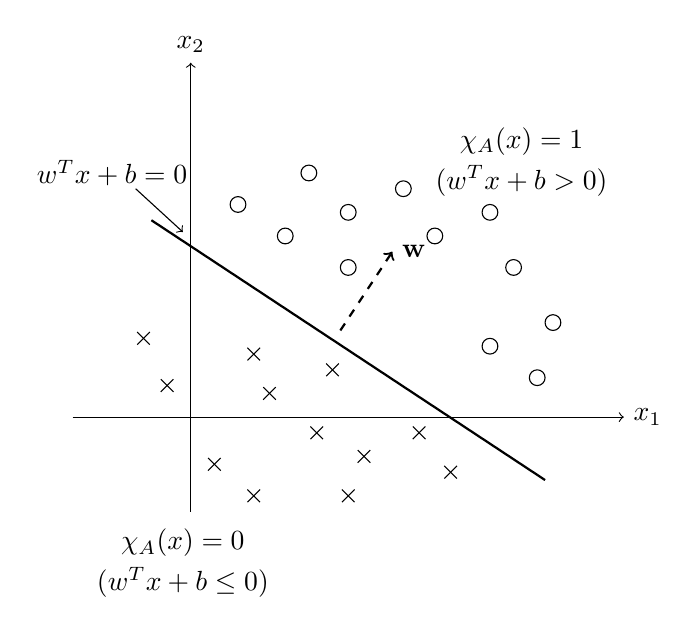
\begin{tikzpicture}
        
    % Ejes
    \draw[->] (0,-1.2) -- (0,4.5) node[above] {$x_2$};
    \draw[->] (-1.5,0) -- (5.5,0) node[right] {$x_1$};

    % Frontera de decisión
    \draw[thick] (-0.5,2.5) -- (4.5,-0.8);
    \node at (-1.0,3.1) {$w^T x + b = 0$};
    \draw[->] (-0.7,2.9) -- (-0.1,2.35);

    % Clase positiva: círculos
    \foreach \x/\y in {
        0.6/2.7, 1.2/2.3, 1.5/3.1, 2.0/2.6, 2.7/2.9,
        3.1/2.3, 3.8/2.6, 4.1/1.9, 2.0/1.9, 3.8/0.9,
        4.6/1.2, 4.4/0.5
    }
    \draw (\x,\y) circle (0.1);

    % Clase negativa: cruces
    \foreach \x/\y in {
        -0.6/1.0, -0.3/0.4, 0.3/-0.6, 0.8/0.8, 1.0/0.3,
        1.6/-0.2, 2.2/-0.5, 2.9/-0.2, 3.3/-0.7, 1.8/0.6,
        0.8/-1.0, 2.0/-1.0
    }{
        \draw (\x-0.08,\y-0.08) -- (\x+0.08,\y+0.08);
        \draw (\x-0.08,\y+0.08) -- (\x+0.08,\y-0.08);
    }

    % Vector normal w
    \draw[dashed,->,thick] (1.9,1.1) -- (2.56,2.10);
    \node[right] at (2.56,2.10) {$\mathbf{w}$};

    % Regiones
    \node at (4.2,3.5) {$\chi_A(x)=1$};
    \node at (4.2,3.0) {$(w^T x + b > 0)$};

    \node at (-0.1,-1.6) {$\chi_A(x)=0$};
    \node at (-0.1,-2.1) {$(w^T x + b \leq 0)$};

    \end{tikzpicture}
    \caption{Ejemplo de clasificador lineal. Los círculos representan la clase positiva y las cruces la clase negativa. La línea representa la frontera de decisión definida por el perceptrón.}
    \label{fig:clasificador_lineal}
\end{figure}

La capa densa generaliza la combinación afín del perceptrón a varias unidades. La no linealidad se aplica después de esta combinación, como se ilustra en la Figura~\ref{fig:capa_red_neuronal}.

\begin{definition}[Capa densa de una red neuronal]
\label{def:capa-densa}
    Sea $L \in \mathbb{N}$ el índice de una capa en una red neuronal.
    Sean:
    $\mathbf{W}^{(L)} \in \mathbb{R}^{n_L \times n_{L-1}}$ la matriz de pesos que conecta la capa $(L-1)$ con la capa $L$, $\mathbf{b}^{(L)} \in \mathbb{R}^{n_L}$ el vector de sesgos, $\sigma : \mathbb{R} \to \mathbb{R}$ una función de activación (aplicada componente a componente).

    Definimos la \textbf{capa $L$-ésima} como la aplicación
    \[
        f^{(L)} : \mathbb{R}^{n_{L-1}} \longrightarrow \mathbb{R}^{n_L},
    \]
    dada por
    \[
        f^{(L)}(\mathbf{x}) = \sigma\!\left(\mathbf{W}^{(L)} \mathbf{x} + \mathbf{b}^{(L)}\right),
    \]
    donde la función de activación $\sigma$ se aplica de manera componente a componente sobre el vector $\mathbf{W}^{(L)} \mathbf{x} + \mathbf{b}^{(L)}$.

    En particular:
    \[
        f^{(0)}(\mathbf{x}) = \mathbf{x}, \qquad \mathbf{x} \in \mathbb{R}^{n_0}.
    \]
\end{definition}

\begin{figure}[H]
    \centering
    \begin{tikzpicture}[x=2.7cm,y=1.6cm,scale=0.80,transform shape]
        % ===== Parámetros visuales =====
        \def\NLm{5}
        \def\yshift{0.4}

        % ===== CAPA (L-1): entradas =====
        \foreach \i [evaluate={\c=int(\i==\NLm); \y=\NLm/2-\i-\c*\yshift; \idx=(\i<\NLm?int(\i):"n_{L-1}");}] in {1,...,\NLm}{
                \node[node in,outer sep=0.6] (Lm-\i) at (0,\y) {$x^{(L-1)}_{\idx}$};
            }
        \path (Lm-\NLm) --++ (0,1+\yshift) node[midway,scale=1.2] {$\vdots$};

        % ===== Bloque lineal: W + b =====
        \node[draw,rounded corners,fill=myblue!5,draw=myblue!20,thick,
            minimum width=1.55cm, minimum height=3.1cm,align=center] (Wb) at (1.25,-0.6)
        {\textbf{W}$^{(L)}$\\\vspace{2mm} $+$\\\vspace{2mm} \textbf{b}$^{(L)}$};

        % ===== Activación sigma =====
        \node[draw,rounded corners,fill=myblue!5,draw=myblue!20,thick,
            minimum width=0.95cm, minimum height=3.1cm, right=0.9cm of Wb] (sigma) {$\sigma$};

        % ===== CAPA (L): salidas  =====

        \foreach \i [evaluate={\idx=(\i<\NLm?int(\i):"n_L");}] in {1,...,\NLm}{
                \node[node hidden] (L-\i)
                at ($(Lm-\i)+(3.50,0)$) {$f^{(L)}_{\idx}$};
            }
        \path (L-\NLm) --++ (0,1+\yshift) node[midway,scale=1.2] {$\vdots$};

        % ===== Cajas de capa =====
        % Caja capa L-1
        \draw[rounded corners]
        ($(Lm-1)+(-0.65,0.65)$) rectangle ($(Lm-\NLm)+(0.65,-0.65)$);
        \node at ($(Lm-1)+(0,1.05)$) {Capa $L-1$};

        % Caja capa L
        \draw[rounded corners]
        ($(L-1)+(-0.75,0.65)$) rectangle ($(L-\NLm)+(0.75,-0.65)$);
        \node at ($(L-1)+(0,1.05)$) {Capa $L$};

        % ===== Conexiones  =====
        \draw[connect] (Lm-1) -- (Wb);
        \draw[connect] (Lm-2) -- (Wb);
        \draw[connect] (Lm-3) -- (Wb);
        \draw[connect] (Lm-4) -- (Wb);
        \draw[connect] (Lm-\NLm) -- (Wb);

        % Wb -> sigma
        \draw[connect] (Wb) -- (sigma);

        % sigma -> todas las neuronas de la capa L
        \foreach \i in {1,...,\NLm}{
                \draw[connect] (sigma) -- (L-\i);
            }

        % ===== Ecuación de la capa =====
        \node at ($ (Wb.south)!0.5!(sigma.south) + (0,-0.8) $) {\small
            $\mathbf{f}^{(L)}=\sigma\!\big(\mathbf{W}^{(L)}\mathbf{x}^{(L-1)}+\mathbf{b}^{(L)}\big)$
        };

    \end{tikzpicture}
    \caption{Capa de una red neuronal con múltiples neuronas en la capa $L$.}
    \label{fig:capa_red_neuronal}
\end{figure}

\begin{observation}
\label{obs:funciones-activacion}
    Una función de activación no lineal $\sigma$ introduce no linealidad en la red neuronal, lo cual es de importancia para que una red pueda aprender representaciones complejas y no lineales de los datos.
    Algunas funciones de activación comunes son:
    \begin{itemize}
        \item \textbf{Función sigmoide}: $\sigma(x) = \frac{1}{1 + e^{-x}}$
        \item \textbf{Función ReLU (Rectified Linear Unit)}: $\sigma(x) = \max(0, x)$
        \item \textbf{Función tanh}: $\sigma(x) = \tanh(x) = \frac{e^x - e^{-x}}{e^x + e^{-x}}$
    \end{itemize}
\end{observation}

La composición de las capas de la Definición~\ref{def:capa-densa} determina la red completa. En este contexto, una red formada por capas densas se denomina también perceptrón multicapa (MLP).

\begin{definition}[Red neuronal]
\label{def:red-neuronal}
    Sea $L \in \mathbb{N}$ el número de capas. Una \textbf{red neuronal} con $L$ capas es una función
    \[
        f(\,\cdot\,;\theta) : \mathbb{R}^{n_0} \longrightarrow \mathbb{R}^{n_L}
    \]
    definida como la composición
    \[
        f(\mathbf{x};\theta) = \bigl(f^{(L)} \circ f^{(L-1)} \circ \dotsb \circ f^{(1)}\bigr)(\mathbf{x}),
    \]
    donde:
    $\mathbf{x} \in \mathbb{R}^{n_0}$ es el vector de entrada, para cada $i \in \{1,\dotsc,L\}$, $f^{(i)} : \mathbb{R}^{n_{i-1}} \to \mathbb{R}^{n_i}$ es la transformación asociada a la $i$-ésima capa, $\theta = (\mathbf{W}^{(i)}, \mathbf{b}^{(i)})_{i=1}^{L}$ es la colección de parámetros de la red (matrices de pesos y vectores de sesgo), $\hat{\mathbf{y}} = f(\mathbf{x};\theta) \in \mathbb{R}^{n_L}$ es la salida de la red.
\end{definition}

La capa $f^{(L)}$ es la capa de salida y las capas $f^{(1)},\ldots,f^{(L-1)}$ son ocultas. La entrada es $\mathbf x$, no una capa con parámetros entrenables. La Figura~\ref{fig:red_neuronal} ilustra el caso de una capa oculta.
\begin{figure}[H]
    \centering
    \begin{tikzpicture}[x=2.7cm,y=1.6cm,scale=0.8,transform shape]

        % ===== Parámetros =====
        \def\NI{3}   % neuronas de entrada
        \def\NH{4}   % neuronas ocultas
        \def\NO{2}   % neuronas de salida
        \def\yshift{0.35}

        % =====================================================
        % CAPA DE ENTRADA
        % =====================================================
        \foreach \i [evaluate={\y=\NI/2-\i;}] in {1,...,\NI}{
                \node[node in] (I-\i) at (0,\y) {$x_{\i}$};
            }

        % Caja entrada
        \draw[rounded corners]
        ($(I-1)+(-0.4,0.6)$) rectangle ($(I-\NI)+(0.4,-0.6)$);
        \node at ($(I-1)+(0,1.0)$) {Entrada};

        % =====================================================
        % CAPA OCULTA
        % =====================================================
        \foreach \i [evaluate={\y=\NH/2-\i;}] in {1,...,\NH}{
                \node[node hidden] (H-\i) at (1.6,\y) {$h_{\i}$};
            }

        % Caja capa oculta
        \draw[rounded corners]
        ($(H-1)+(-0.4,0.6)$) rectangle ($(H-\NH)+(0.4,-0.6)$);
        \node at ($(H-1)+(0,1.0)$) {Capa oculta};

        % =====================================================
        % CAPA DE SALIDA
        % =====================================================
        \foreach \i [evaluate={\y=\NO/2-\i;}] in {1,...,\NO}{
                \node[node hidden] (O-\i) at (3.2,\y) {$y_{\i}$};
            }

        % Caja salida
        \draw[rounded corners]
        ($(O-1)+(-0.4,0.6)$) rectangle ($(O-\NO)+(0.4,-0.6)$);
        \node at ($(O-1)+(0,1.0)$) {Salida};

        % =====================================================
        % CONEXIONES
        % =====================================================

        % Entrada -> Oculta
        \foreach \i in {1,...,\NI}{
                \foreach \j in {1,...,\NH}{
                        \draw[connect] (I-\i) -- (H-\j);
                    }
            }

        % Oculta -> Salida
        \foreach \i in {1,...,\NH}{
                \foreach \j in {1,...,\NO}{
                        \draw[connect] (H-\i) -- (O-\j);
                    }
            }

    \end{tikzpicture}
    \caption{Ejemplo de red neuronal con una capa oculta.}
    \label{fig:red_neuronal}
\end{figure}


\subsection{Entrenamiento de redes neuronales}

Entrenar una red consiste en ajustar sus parámetros a partir de observaciones etiquetadas. Se distinguirán la pérdida de una predicción, su promedio en la distribución de datos y el promedio calculable sobre el conjunto de entrenamiento. Esta distinción permite interpretar la evaluación de clasificación del Capítulo~\ref{cap:resultados} sin identificar el error de entrenamiento con el comportamiento en datos no utilizados para ajustar el modelo.

\begin{definition}[Conjunto de entrenamiento]
\label{def:conjunto-entrenamiento}
    Sea $\mathcal{X}$ el espacio de entrada (o espacio de características) y sea $\mathcal{Y}$ el espacio de salida (o espacio de etiquetas). 
    
    Un \textbf{conjunto de datos de entrenamiento} es una colección finita de $N$ observaciones empíricas, denotada por
    \[
        \mathcal{D} = \{(x_1, y_1), (x_2, y_2), \dots, (x_N, y_N)\} = \{(x_i,y_i)\}_{i=1}^N,
    \]
    donde cada par $(x_i, y_i) \in \mathcal{X} \times \mathcal{Y}$ representa un ejemplo individual. En este contexto, $x_i$ corresponde a las características observadas del $i$-ésimo ejemplo y $y_i$ es su valor verdadero o etiqueta asociada.
\end{definition}

En la tarea de clasificación de superficies, cada $x_i$ representa una superficie mediante los datos que recibe el modelo, y $y_i$ es la etiqueta de esa observación. El muestreo del Capítulo~\ref{cap:muestreo} modifica la representación de $x_i$; reducir sus nodos no equivale a retirar observaciones de $\mathcal D$.

\begin{definition}[Función de pérdida]
\label{def:funcion-perdida}
Sea $\mathcal{Y}$ el espacio de valores verdaderos y sea
$\widehat{\mathcal{Y}}$ el espacio de predicciones de un modelo.

Una \textbf{función de pérdida} es una función
\[
    \ell:\mathcal{Y}\times\widehat{\mathcal{Y}}
    \longrightarrow \mathbb{R}_{\geq 0},
\]
donde $\ell(y,\hat{y})$ cuantifica la discrepancia entre el valor verdadero
$y\in\mathcal{Y}$ y una predicción
$\hat{y}\in\widehat{\mathcal{Y}}$.

En particular, si
\[
    f(\,\cdot\,;\theta):\mathcal{X}\longrightarrow
    \widehat{\mathcal{Y}}
\]
es una red neuronal parametrizada por $\theta\in\Theta$, donde $\Theta$ es el espacio de parámetros, entonces la pérdida
asociada a un dato de entrenamiento $(x_i,y_i)$ está dada por
\[
    \ell\bigl(y_i,f(x_i;\theta)\bigr).
\]

\end{definition}

La pérdida puntual se promedia respecto de una distribución de probabilidad para formular el objetivo poblacional del aprendizaje. Se denota esta distribución por $\mathbb P$, reservando $\mathcal D$ para la colección finita de observaciones.

\begin{definition}[Función de riesgo]
\label{def:riesgo-esperado}
Sea $\mathbb P$ una distribución de probabilidad sobre $\mathcal X\times\mathcal Y$. Para una pérdida $\ell$ y un predictor $f(\,\cdot\,;\theta)$, se define el \textbf{riesgo esperado} por
\[
\mathcal R(\theta)=\mathbb E_{(x,y)\sim\mathbb P}\bigl[\ell(y,f(x;\theta))\bigr],
\]
siempre que la pérdida compuesta sea medible e integrable. Bajo esta condición, $\mathcal R:\Theta\to\mathbb R_{\geq0}$ cuantifica la pérdida promedio sobre la distribución de datos.
\end{definition}

Como la distribución $\mathbb P$ es desconocida, se emplea un promedio sobre las observaciones disponibles.

\begin{definition}[Función de riesgo empírico]
\label{def:riesgo-empirico}
Dado el conjunto de entrenamiento $\mathcal D=\{(x_i,y_i)\}_{i=1}^{N}$, con $N\geq1$, el \textbf{riesgo empírico} es
\[
\widehat{\mathcal R}(\theta)=\frac1N\sum_{i=1}^{N}\ell\bigl(y_i,f(x_i;\theta)\bigr).
\]
El problema de minimización del riesgo empírico consiste en buscar parámetros que reduzcan $\widehat{\mathcal R}$ sobre $\Theta$.
\end{definition}


La pérdida $\ell$ corresponde a una observación, mientras que $\mathcal R$ y $\widehat{\mathcal R}$ son promedios distintos. Reducir la pérdida de entrenamiento no garantiza obtener buena clasificación en datos nuevos. Para ajustar los parámetros se utilizan métodos de optimización que, cuando existen las derivadas necesarias, se apoyan en el gradiente.

\begin{definition}[Gradiente]
\label{def:gradiente}
Sea $f:\Omega\to\mathbb R$, con $\Omega\subseteq\mathbb R^n$ abierto, diferenciable en $x_0\in\Omega$. Su \textbf{gradiente} en $x_0$ es el vector columna
\[
\nabla f(x_0)=\left(\frac{\partial f}{\partial x_1}(x_0),\ldots,\frac{\partial f}{\partial x_n}(x_0)\right)^T.
\]
\end{definition}
El producto $\nabla f(x_0)^T d$ da la derivada direccional en la dirección $d$. Si el gradiente es distinto de cero, su opuesto es una dirección de descenso local.

\begin{definition}[Descenso por gradiente]
\label{def:descenso-gradiente}
    Sea $J : \Theta \to \mathbb{R}$ una función diferenciable, denominada \textit{función objetivo}, donde $\Theta=\mathbb{R}^n$ representa el espacio de parámetros sin restricciones.
    Dado un valor inicial $\theta_0 \in \Theta$ y una tasa de aprendizaje $\eta > 0$, el \textit{método de descenso por gradiente} genera una sucesión
    $\{ \theta_k \}_{k \in \mathbb{N}}$ definida recursivamente por
    \[
        \theta_{k+1} = \theta_k - \eta \, \nabla_\theta J(\theta_k),
    \]
    donde $\nabla_\theta J(\theta_k)$ denota el gradiente de $J$ evaluado en $\theta_k$.
\end{definition}

Notamos que el descenso por gradiente es un método iterativo que busca minimizar una función objetivo $J(\theta)$ ajustando los parámetros $\theta$ en la dirección opuesta al gradiente de la función. La tasa de aprendizaje $\eta$ controla el tamaño de los pasos que se dan en cada iteración, lo que afecta el comportamiento del método. La actualización no garantiza por sí sola convergencia ni descenso para cualquier valor de $\eta$.


\begin{figure}[H]
    \centering
    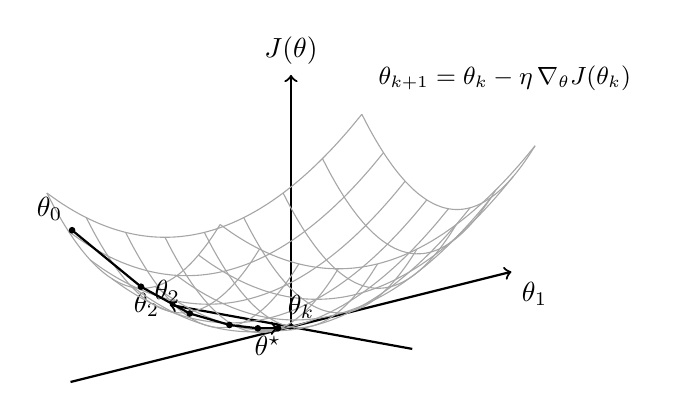
\begin{tikzpicture}[scale=1.0]

        % ===============================
        % Proyección 3D oblicua manual
        % ===============================
        \def\a{0.55}
        \def\b{0.25}
        \def\c{0.10}

        % Macro de proyección segura
        \providecommand{\Proj}[3]{%
            ({#1 - \a*#2},{\b*#1 + \c*#2 + #3})%
        }

        % ===============================
        % Ejes (espacio de parámetros)
        % ===============================
        \draw[->, thick] \Proj{-2.8}{0}{0} -- \Proj{2.8}{0}{0} node[below right] {$\theta_1$};
        \draw[->, thick] \Proj{0}{-2.8}{0} -- \Proj{0}{2.8}{0} node[left] {$\theta_2$};
        \draw[->, thick] \Proj{0}{0}{0} -- \Proj{0}{0}{3.2} node[above] {$J(\theta)$};

        % Mínimo global
        \fill \Proj{0}{0}{0} circle (1.2pt);
        \node[below left] at \Proj{0}{0}{0} {$\theta^\star$};

        % ===============================
        % Superficie: función objetivo
        % J(\theta) = (theta_1^2 + theta_2^2)/4
        % ===============================

        % Curvas theta_1 = const
        \foreach \t in {-2,-1.5,-1,-0.5,0,0.5,1,1.5,2}{
                \draw[black!35]
                plot[smooth,variable=\s,domain=-2:2,samples=25]
                (\Proj{\t}{\s}{(\t*\t+\s*\s)/4});
            }

        % Curvas theta_2 = const
        \foreach \s in {-2,-1.5,-1,-0.5,0,0.5,1,1.5,2}{
                \draw[black!35]
                plot[smooth,variable=\t,domain=-2:2,samples=25]
                (\Proj{\t}{\s}{(\t*\t+\s*\s)/4});
            }

        % ===============================
        % Descenso por gradiente: sucesión {theta_k}
        % ===============================
        \draw[->, thick]
        \Proj{-1.9}{1.6}{(1.9*1.9+1.6*1.6)/4} --
        \Proj{-1.3}{1.1}{(1.3*1.3+1.1*1.1)/4} --
        \Proj{-0.9}{0.7}{(0.9*0.9+0.7*0.7)/4} --
        \Proj{-0.55}{0.42}{(0.55*0.55+0.42*0.42)/4} --
        \Proj{-0.30}{0.22}{(0.30*0.30+0.22*0.22)/4} --
        \Proj{-0.12}{0.08}{(0.12*0.12+0.08*0.08)/4};

        % Puntos de iteración
        \foreach \x/\y in {
                -1.9/1.6,
                -1.3/1.1,
                -0.9/0.7,
                -0.55/0.42,
                -0.30/0.22,
                -0.12/0.08}{
                \fill \Proj{\x}{\y}{(\x*\x+\y*\y)/4} circle (1.2pt);
            }

        % Etiquetas de la sucesión
        \node[above left]  at \Proj{-1.9}{1.6}{(1.9*1.9+1.6*1.6)/4} {$\theta_0$};
        \node[above left]  at \Proj{-0.9}{0.7}{(0.9*0.9+0.7*0.7)/4} {$\theta_2$};
        \node[above right] at \Proj{-0.12}{0.08}{(0.12*0.12+0.08*0.08)/4} {$\theta_k$};

        % ===============================
        % Regla de actualización (definición)
        % ===============================
        \node[align=left] at \Proj{2.0}{-1.4}{2.8} {\small
            $\displaystyle
                \theta_{k+1} = \theta_k - \eta\,\nabla_\theta J(\theta_k)$
        };

    \end{tikzpicture}
    \caption{Ilustración geométrica del método de descenso por gradiente aplicado a una función objetivo $J : \Theta \subseteq \mathbb{R}^n \to \mathbb{R}$.}
    \label{fig:descenso_gradiente}
\end{figure}

De esta forma podemos describir formalmente el algoritmo de actualización  de parámetros por medio del descenso de gradiente.

\begin{algorithm}[H]
\caption{Actualización por descenso del gradiente}\label{alg:descenso-gradiente}
\begin{algorithmic}[1]
\Require Objetivo diferenciable $J:\mathbb R^n\to\mathbb R$, $T\geq1$, $\eta>0$, $\theta^{(0)}$
\For{$t=0,\ldots,T-1$}
    \State $g\gets\nabla J(\theta^{(t)})$
    \If{$g=0$}
        \State \Return $\theta^{(t)}$
    \EndIf
    \State $\theta^{(t+1)}\gets\theta^{(t)}-\eta g$
\EndFor
\State \Return $\theta^{(T)}$
\end{algorithmic}
\end{algorithm}

En el entrenamiento puede tomarse $J=\widehat{\mathcal R}$. El Algoritmo~\ref{alg:descenso-gradiente} presupone que se conoce su gradiente; la retropropagación permite calcularlo a través de las capas sin ser, por sí misma, una regla de actualización de parámetros.

\subsection{Backpropagation}
La \textbf{retropropagación} (\textit{backpropagation}) aplica la regla de la cadena para calcular las derivadas de la pérdida respecto de los parámetros. Se separan el cálculo de activaciones, la propagación de derivadas y la actualización mediante un optimizador. La Figura~\ref{fig:backpropagation} ilustra estos recorridos para una red con una capa oculta.

\begin{figure}[H]
    \centering
    \begin{tikzpicture}[x=2.7cm,y=1.6cm,scale=0.95,transform shape]

        % =====================================================
        % Estilos locales adicionales (compatibles con tu preámbulo)
        % =====================================================
        \tikzset{
        back/.style={-{Latex[length=4,width=3.5]},thick,red!80!black},
        note/.style={font=\scriptsize,align=center},
        labw/.style={font=\scriptsize,sloped,inner sep=1pt,fill=white},
        labd/.style={font=\scriptsize,sloped,inner sep=1pt,fill=white,text=red!80!black}
        }

        % =====================================================
        % NODOS (coordenadas explícitas)
        % =====================================================
        % Entrada
        \node[node in]     (x1) at (0, 0.55) {$x_{1}$};
        \node[node in]     (x2) at (0,-0.55) {$x_{2}$};

        % Capa oculta (Capa 1)
        \node[node hidden] (h1) at (1.5, 0.55) {$h^{(1)}_{1}$};
        \node[node hidden] (h2) at (1.5,-0.55) {$h^{(1)}_{2}$};

        % Salida
        \node[node out]    (yhat) at (3.0, 0.0) {$\hat{y}=h^{(2)}$};

        % Pérdida
        \node[node out]    (L)    at (4.4, 0.0) {$\ell$};

        % =====================================================
        % FORWARD PASS (azul)
        % Nota: estas flechas no chocan con backprop en tu captura,
        % pero dejamos consistencia con curvas suaves.
        % =====================================================
        \draw[connect arrow, bend left=10]
        (x1) to node[pos=0.35,above,labw] {$w^{(1)}_{11}$} (h1);

        \draw[connect arrow, bend left=10]
        (x1) to node[pos=0.35,below,labw] {$w^{(1)}_{21}$} (h2);

        \draw[connect arrow, bend left=10]
        (x2) to node[pos=0.35,above,labw] {$w^{(1)}_{12}$} (h1);

        \draw[connect arrow, bend left=10]
        (x2) to node[pos=0.35,below,labw] {$w^{(1)}_{22}$} (h2);

        % =====================================================
        % CLAVE: Separación forward/back en capa oculta <-> salida
        %   - Forward sale/entra "arriba"
        %   - Backprop sale/entra "abajo"
        %   usando (yshift) en los anclajes + bend
        % =====================================================

        % Forward (arriba)
        \draw[connect arrow, bend left=14]
        ([yshift=3pt]h1.east) to node[pos=0.35,above,labw] {$w^{(2)}_{1}$} ([yshift=3pt]yhat.west);

        \draw[connect arrow, bend left=14]
        ([yshift=-3pt]h2.east) to node[pos=0.35,below,labw] {$w^{(2)}_{2}$} ([yshift=-3pt]yhat.west);

        % Forward yhat -> L (arriba)
        \draw[connect arrow, bend left=12]
        ([yshift=3pt]yhat.east) to ([yshift=3pt]L.west);

        % =====================================================
        % BACKPROP (rojo) con anclajes desplazados (abajo)
        % =====================================================

        % Delta de salida (abajo) L -> yhat
        \draw[back, bend right=12]
        ([yshift=-3pt]L.west) to
        node[pos=0.55,below,note,fill=white,inner sep=1pt,text=red!80!black]
        {$\delta^{(2)}$}
        ([yshift=-3pt]yhat.east);

        % Deltas a capa oculta (abajo/arriba para evitar cruces)
        \draw[back, bend right=14]
        ([yshift=-3pt]yhat.west) to node[pos=0.65,below,labd] {$\delta^{(1)}_{1}$} ([yshift=-3pt]h1.east);

        \draw[back, bend right=14]
        ([yshift=3pt]yhat.west) to node[pos=0.65,above,labd] {$\delta^{(1)}_{2}$} ([yshift=3pt]h2.east);

        % =====================================================
        % Anotaciones de capas
        % =====================================================
        \node[note] at (0,   1.20) {Entrada};
        \node[note] at (1.5, 1.20) {Capa 1};
        \node[note] at (3.0, 1.20) {Salida};
        \node[note] at (4.4, 1.20) {Pérdida};

        % =====================================================
        % Ecuaciones 
        % =====================================================
        \node[font=\scriptsize,align=left] at (2.2,-1.70) {%
            \textbf{Forward:}\\[-1pt]
            $z^{(1)} = W^{(1)}x + b^{(1)},\quad h^{(1)}=\sigma(z^{(1)})$\\
            $z^{(2)} = W^{(2)}h^{(1)} + b^{(2)},\quad \hat{y}=h^{(2)}=\sigma(z^{(2)})$\\[4pt]
            \textbf{Backprop:}\\[-1pt]
            $\delta^{(2)}=\nabla_{h^{(2)}}\ell\odot\sigma'(z^{(2)})$\\
            $\delta^{(1)}=(W^{(2)})^{T}\delta^{(2)}\odot\sigma'(z^{(1)})$\\[4pt]
            $\displaystyle
                \frac{\partial\ell}{\partial W^{(2)}}=\delta^{(2)}(h^{(1)})^{T},\quad
                \frac{\partial\ell}{\partial W^{(1)}}=\delta^{(1)}x^{T}$
        };

        \node[font=\scriptsize] at (3.8,-1.05)
        {$W^{(l)} \leftarrow W^{(l)} - \eta\,\nabla_{W^{(l)}}\ell$};

        % =====================================================
        % Leyenda
        % =====================================================
        \draw[connect arrow] (0.2,1.65) -- (0.65,1.65);
        \node[font=\scriptsize,anchor=west] at (0.72,1.65) {Forward};

        \draw[back] (1.55,1.65) -- (2.00,1.65);
        \node[font=\scriptsize,anchor=west] at (2.07,1.65) {Backprop};

    \end{tikzpicture}
    \caption{Propagación de activaciones hacia la salida (azul) y de derivadas hacia las capas anteriores (rojo). La actualización utiliza los gradientes calculados.}
    \label{fig:backpropagation}
\end{figure}
\newpage
\begin{definition}[Gradiente de la función de riesgo empírico]
\label{def:gradiente-riesgo-empirico}
Se agrupan las entradas de las matrices de pesos y los sesgos en un vector $\theta\in\mathbb R^p$. Si las pérdidas compuestas son diferenciables respecto de este vector, entonces
\[
\nabla_\theta\widehat{\mathcal R}(\theta)
=\frac1N\sum_{i=1}^{N}\nabla_\theta\ell\bigl(y_i,f(x_i;\theta)\bigr).
\]
Si, además, la red es diferenciable respecto de sus parámetros y la pérdida respecto de la predicción, la regla de la cadena da
\[
\nabla_\theta\ell\bigl(y_i,f(x_i;\theta)\bigr)
=\bigl(D_\theta f(x_i;\theta)\bigr)^T
\left.\nabla_{\hat y}\ell(y_i,\hat y)\right|_{\hat y=f(x_i;\theta)},
\]
donde $D_\theta f\in\mathbb R^{n_L\times p}$ es el jacobiano respecto de todos los parámetros de la red.
\end{definition}

La Definición~\ref{def:gradiente-riesgo-empirico} permite calcular el gradiente por observación y promediarlo. Para obtenerlo sin formar el jacobiano completo, se recorre la composición de capas en sentido inverso. A continuación se supone que cada activación se aplica componente a componente y es diferenciable en las preactivaciones consideradas.

\noindent\textbf{Propagación hacia delante.}
Para una observación $(\mathbf x,y)$ se fija $\mathbf h^{(0)}=\mathbf x$. Para cada capa $l=1,\ldots,L$, se calculan la preactivación y la activación:
\[
\mathbf z^{(l)}=\mathbf W^{(l)}\mathbf h^{(l-1)}+\mathbf b^{(l)},
\qquad
\mathbf h^{(l)}=\sigma(\mathbf z^{(l)}).
\]
La pérdida puntual es $\ell(y,\mathbf h^{(L)})$.

\noindent\textbf{Propagación hacia atrás.}
Se denota por $\delta^{(l)}$ el gradiente de esta pérdida respecto de $\mathbf z^{(l)}$. Con $\odot$ para el producto componente a componente, se obtiene
\[
\delta^{(L)}=\nabla_{\mathbf h^{(L)}}\ell(y,\mathbf h^{(L)})
\odot\sigma'(\mathbf z^{(L)}),
\]
y, para $l=L-1,\ldots,1$,
\[
\delta^{(l)}=(\mathbf W^{(l+1)})^T\delta^{(l+1)}
\odot\sigma'(\mathbf z^{(l)}).
\]
Los gradientes de los parámetros de \emph{todas} las capas, incluida la de salida, son
\[
\nabla_{\mathbf W^{(l)}}\ell=\delta^{(l)}(\mathbf h^{(l-1)})^T,
\qquad
\nabla_{\mathbf b^{(l)}}\ell=\delta^{(l)},\qquad l=1,\ldots,L.
\]
El primer producto es exterior y tiene las dimensiones de $\mathbf W^{(l)}$. Todos los gradientes se calculan antes de modificar los parámetros. Si se utiliza ReLU, no existe derivada en cero; el procedimiento requiere una convención en ese punto, por ejemplo asignar el valor cero. Para activaciones vectoriales no separables debe utilizarse su jacobiano, en lugar del producto componente a componente anterior.

El Algoritmo~\ref{alg:backpropagation} combina estas operaciones con una actualización por observación. Esta variante se denomina descenso estocástico del gradiente cuando las observaciones se seleccionan aleatoriamente. Promediar los gradientes de todas las observaciones recupera el gradiente del riesgo empírico; promediar sólo un lote da la actualización por minilotes.

\begin{algorithm}[H]
\caption{Retropropagación y actualización por observación}
\label{alg:backpropagation}
\begin{algorithmic}[1]
\Require Datos $\mathcal D$, capas $L$, épocas $T$, tasa $\eta>0$ y parámetros iniciales
\For{cada época $t=1,\ldots,T$}
    \For{cada observación $(\mathbf x,y)$ en el orden elegido para la época}
        \State $\mathbf h^{(0)}\gets\mathbf x$
        \For{$l=1,\ldots,L$}
            \State $\mathbf z^{(l)}\gets\mathbf W^{(l)}\mathbf h^{(l-1)}+\mathbf b^{(l)}$
            \State $\mathbf h^{(l)}\gets\sigma(\mathbf z^{(l)})$
        \EndFor
        \State Calcular $\ell(y,\mathbf h^{(L)})$
        \State $\delta^{(L)}\gets\nabla_{\mathbf h^{(L)}}\ell(y,\mathbf h^{(L)})\odot\sigma'(\mathbf z^{(L)})$
        \For{$l=L-1,\ldots,1$}
            \State $\delta^{(l)}\gets(\mathbf W^{(l+1)})^T\delta^{(l+1)}\odot\sigma'(\mathbf z^{(l)})$
        \EndFor
        \For{$l=1,\ldots,L$}
            \State $g_W^{(l)}\gets\delta^{(l)}(\mathbf h^{(l-1)})^T$; $g_b^{(l)}\gets\delta^{(l)}$
        \EndFor
        \For{$l=1,\ldots,L$}
            \State $\mathbf W^{(l)}\gets\mathbf W^{(l)}-\eta g_W^{(l)}$
            \State $\mathbf b^{(l)}\gets\mathbf b^{(l)}-\eta g_b^{(l)}$
        \EndFor
    \EndFor
\EndFor
\end{algorithmic}
\end{algorithm}

Estos mecanismos de entrenamiento se aplican también a las transformaciones aprendibles de las arquitecturas posteriores. Lo que cambia entre modelos es, entre otros aspectos, la forma de compartir parámetros y combinar los datos. La convolución permite introducir estas ideas sobre una cuadrícula antes de considerar vecindarios en gráficas.

\section{Redes convolucionales CNN}
Una \textbf{red neuronal convolucional (CNN)} procesa datos en cuadrículas mediante operaciones locales con parámetros compartidos. Se estudian como antecedente de la agregación de información y de las simetrías de los modelos sobre gráficas, siguiendo \cite{Goodfellow-et-al-2016}. La exposición distingue la convolución matemática de la operación habitualmente implementada en las capas y conserva las convenciones necesarias para interpretar los esquemas.

\subsection{Operación de convolución}

Para entender las redes convolucionales, es esencial comprender primero la operación matemática de la convolución. A continuación, se presentan las definiciones clave relacionadas con la convolución en diferentes contextos.
\begin{definition}[Convolución]
\label{def:convolucion}
Sean $x,w\in L^1(\mathbb R)$, es decir, funciones medibles absolutamente integrables. Su \textbf{convolución} se define por
\[
(x\ast w)(t)=\int_{\mathbb R}x(a)w(t-a)\,da
\]
en los puntos donde la integral converge absolutamente. Para estas funciones la expresión está definida casi en todas partes y determina una función de $L^1(\mathbb R)$.
\end{definition}

En el contexto de las redes neuronales convolucionales, el primer término (la función $x$) se refiere a la entrada, y el segundo término (la función $w$) es el kernel o filtro.

Dado que en muchos escenarios, el tipo de datos es discreto, se maneja otro tipo de convolución, llamada convolución discreta.
\begin{definition}[Convolución discreta]
\label{def:convolucion-discreta}
    Sean $x, w : \mathbb{Z} \to \mathbb{R}$ dos sucesiones absolutamente sumables.
    La \textbf{convolución discreta} de $x$ y $w$, denotada por $x \ast w$, es la sucesión
    \[
        (x \ast w) : \mathbb{Z} \to \mathbb{R}
    \]
    definida, para todo $n \in \mathbb{Z}$, por
    \[
        (x \ast w)(n) = \sum_{a=-\infty}^{\infty} x(a)\, w(n - a),
    \]
    siempre que dicha serie sea convergente.
\end{definition}

Finalmente, para el uso particular del procesamiento de imágenes en dos dimensiones, podemos utilizar la convolución discreta en dos dimensiones.

\begin{definition}[Convolución discreta en dos dimensiones]
\label{def:convolucion-discreta-2d}
    Sean $\mathbf{I}, \mathbf{K} : \mathbb{Z}^2 \to \mathbb{R}$ dos funciones (o matrices discretas) absolutamente sumables.
    La \textbf{convolución discreta bidimensional} de $\mathbf{I}$ y $\mathbf{K}$, denotada por $\mathbf{I} \ast \mathbf{K}$, es la función
    \[
        (\mathbf{I} \ast \mathbf{K}) : \mathbb{Z}^2 \to \mathbb{R}
    \]
    definida, para todo $(i,j) \in \mathbb{Z}^2$, por
    \[
        (\mathbf{I} \ast \mathbf{K})(i,j) = \sum_{m=-\infty}^{\infty} \sum_{n=-\infty}^{\infty}
        \mathbf{I}(m,n)\, \mathbf{K}(i - m, j - n),
    \]
    siempre que la doble suma sea convergente.
\end{definition}

\begin{observation}
\label{obs:conmutatividad-convolucion}
    La operación de convolución es conmutativa, es decir,
    \[
        \mathbf{I} \ast \mathbf{K} = \mathbf{K} \ast \mathbf{I}.
    \]
\end{observation}

\begin{proof}
La sumabilidad absoluta permite efectuar el cambio de índices $u=i-m$, $v=j-n$. Para cada $(i,j)\in\mathbb Z^2$,
\[
(\mathbf I\ast\mathbf K)(i,j)
=\sum_{u,v\in\mathbb Z}\mathbf I(i-u,j-v)\mathbf K(u,v)
=(\mathbf K\ast\mathbf I)(i,j).
\]
\end{proof}

La Figura~\ref{fig:convolucion2D} ilustra el filtrado local mediante un kernel simétrico respecto de su centro. El cálculo usa ventanas válidas y, por esa simetría, coincide con la correlación cruzada que se distinguirá de la convolución al definir los filtros.

\begin{figure}[ht]
    \centering
    \begin{tikzpicture}[
    2d-arr/.style={matrix of nodes, row sep=-\pgflinewidth, column sep=-\pgflinewidth, nodes={draw}}
  ]

  \matrix (mtr) [2d-arr] {
  0 & 1 & 1 & |[fill=orange!30]| 1 & |[fill=orange!30]| 0 & |[fill=orange!30]| 0 & 0\\
  0 & 0 & 1 & |[fill=orange!30]| 1 & |[fill=orange!30]| 1 & |[fill=orange!30]| 0 & 0\\
  0 & 0 & 0 & |[fill=orange!30]| 1 & |[fill=orange!30]| 1 & |[fill=orange!30]| 1 & 0\\
  0 & 0 & 0 & 1 & 1 & 0 & 0\\
  0 & 0 & 1 & 1 & 0 & 0 & 0\\
  0 & 1 & 1 & 0 & 0 & 0 & 0\\
  1 & 1 & 0 & 0 & 0 & 0 & 0\\
  };

  \node[below=of mtr-5-4] {$\mathbf I$};

  \node[right=0.2em of mtr] (str) {$*$};

  \matrix (K) [2d-arr, right=0.2em of str, nodes={draw, fill=teal!30}] {
    1 & 0 & 1 \\
    0 & 1 & 0 \\
    1 & 0 & 1 \\
  };
  \node[below=of K-3-2] {$\mathbf K$};

  \node[right=0.2em of K] (eq) {$=$};

  \matrix (ret) [2d-arr, right=0.2em of eq] {
  1 & 4 & 3 & |[fill=blue!80!black!30]| 4 & 1\\
  1 & 2 & 4 & 3 & 3\\
  1 & 2 & 3 & 4 & 1\\
  1 & 3 & 3 & 1 & 1\\
  3 & 3 & 1 & 1 & 0\\
  };
  \node[below=of ret-4-3] {$\mathbf{I * K}$};

  \draw[dashed, teal] (mtr-1-6.north east) -- (K-1-1.north west);
  \draw[dashed, teal] (mtr-3-6.south east) -- (K-3-1.south west);

  \draw[dashed, blue!80!black] (K-1-3.north east) -- (ret-1-4.north west);
  \draw[dashed, blue!80!black] (K-3-3.south east) -- (ret-1-4.south west);

  \foreach \i in {1,2,3} {
      \foreach \j in {4,5,6} {
          \node[font=\tiny, scale=0.6, shift={(-1.2ex,-2ex)}] at (mtr-\i-\j) {$\times \pgfmathparse{int(mod(\i+\j,2))}\pgfmathresult$};
        }
    }

\end{tikzpicture}
    \caption{Ilustración de la operación de convolución  $\mathbf{I}$ y un kernel $\mathbf{K}$.}
    \label{fig:convolucion2D}
\end{figure}


\subsection{Propiedades de convolución}
Una de las propiedades más importantes de la operación de convolución es su comportamiento bajo ciertas transformaciones, específicamente la invarianza y la equivarianza. Estas propiedades son fundamentales para entender cómo las redes convolucionales pueden aprender características relevantes de los datos de entrada.
A continuación, se presentan las definiciones formales de invarianza y equivarianza.

\begin{definition}[Invarianza]
\label{def:invarianza}
    Sea $f: \mathbf{X} \longrightarrow \mathbf{Y}$ una función, $\mathbf{T}$ una transformación en $\mathbf{X}$. Se dice que una función $f$ es invariante bajo $\mathbf{T}$ si:
    \[
        f\left(\mathbf{T}(x)\right) = f(x) , \hspace{1cm} \forall x \in \mathbf{X}
    \]
\end{definition}

\begin{definition}[Equivarianza]
\label{def:equivarianza}
Sean $f:\mathbf X\to\mathbf Y$ y transformaciones $\mathbf T_{\mathbf X}:\mathbf X\to\mathbf X$ y $\mathbf T_{\mathbf Y}:\mathbf Y\to\mathbf Y$. Se dice que $f$ es \textbf{equivariante} respecto de estas transformaciones si
\[
f(\mathbf T_{\mathbf X}(x))=\mathbf T_{\mathbf Y}(f(x)),\qquad x\in\mathbf X.
\]
\end{definition}
De lo anterior podemos observar que la invarianza implica que la salida de la función no cambia cuando se aplica una transformación a la entrada, mientras que la equivarianza implica que la transformación de la entrada se refleja de manera consistente en la salida.
A continuación, demostraremos que la operación de convolución es equivariante bajo traslaciones.

\begin{teorema}[Equivarianza de la convolución bajo traslaciones]
\label{teo:convolucion-traslaciones}

    Sea $f, k \in L^1(\mathbb{R})$ y sea $\mathbf{T}_a$ el operador de traslación definido por
    \[
        (\mathbf{T}_a f)(x) = f(x - a), \quad a \in \mathbb{R}.
    \]
    Entonces, para casi todo $x \in \mathbb{R}$, se cumple que
    \[
        (\mathbf{T}_a f \ast k)(x) = (f \ast k)(x - a).
    \]
\end{teorema}

\begin{proof}
    Por definición de la convolución en $\mathbb{R}$, tenemos que
    \[
        (\mathbf{T}_a f \ast k)(x) = \int_{\mathbb{R}} (\mathbf{T}_a f)(t)\, k(x - t)\,
        dt.
    \]
    Sustituyendo la definición de la traslación, se obtiene
    \[
        (\mathbf{T}_a f \ast k)(x) = \int_{\mathbb{R}} f(t - a)\, k(x - t)\, dt.
    \]
    Haciendo el cambio de variable $u = t - a$, de modo que $du = dt$ y $t = u + a$, se sigue que
    \[
        (\mathbf{T}_a f \ast k)(x) = \int_{\mathbb{R}} f(u)\, k(x - (u + a))\, du.
    \]
    Reordenando los términos en el argumento de $k$, obtenemos
    \[
        (\mathbf{T}_a f \ast k)(x) = \int_{\mathbb{R}} f(u)\, k((x - a) - u)\, du.
    \]
    Por la definición de la convolución, esto equivale a
    \[
        (f \ast k)(x - a) = \int_{\mathbb{R}} f(u)\, k((x - a) - u)\, du.
    \]
    Por lo tanto,
    \[
        (\mathbf{T}_a f \ast k)(x) = (f \ast k)(x - a), \quad \text{para casi todo }x\in\mathbb R.
    \]
\end{proof}
El Teorema~\ref{teo:convolucion-traslaciones} expresa equivarianza: trasladar la entrada traslada el resultado de la convolución. No implica que toda CNN sea invariante o equivariante ante cualquier traslación, pues el tratamiento de bordes, el paso del filtro y las capas posteriores pueden modificar esta propiedad. La misma distinción entre una salida que se transforma y una salida que permanece igual se retomará para las permutaciones de nodos.

\subsection{Filtros y mapas de características}

En el contexto de las redes neuronales convolucionales, los \textbf{filtros} (o kernels) son matrices de pesos que se utilizan para extraer características locales de los datos de entrada mediante la operación de convolución. A continuación, se presentan las definiciones clave relacionadas con los filtros y los mapas de características.

\begin{definition}[Kernel o filtro]
\label{def:kernel}
Para una entrada $\mathbf X\in\mathbb R^{m\times n}$, un \textbf{kernel} es una matriz de pesos $\mathbf K\in\mathbb R^{h\times w}$, con $1\leq h\leq m$ y $1\leq w\leq n$. La operación local sin invertir el filtro es la \textbf{correlación cruzada}, que se denota aquí por $\star$:
\[
(\mathbf X\star\mathbf K)(i,j)
=\sum_{u=1}^{h}\sum_{v=1}^{w}\mathbf X(i+u-1,j+v-1)\mathbf K(u,v),
\]
para $1\leq i\leq m-h+1$ y $1\leq j\leq n-w+1$.
\end{definition}

El desplazamiento de índices corresponde a una enumeración desde uno y sitúa la esquina superior izquierda de la ventana en $(i,j)$. Muchas capas llamadas convolucionales utilizan esta correlación \cite{Goodfellow-et-al-2016}; se reserva $\ast$ para la convolución matemática. Los filtros aprendidos no tienen que ser simétricos ni estar normalizados para sumar uno. Sus $h\times w$ dimensiones espaciales determinan $hw$ coeficientes por canal.

\begin{definition}[Mapa de características]
\label{def:mapa-caracteristicas}
Para $\mathbf I\in\mathbb R^{m\times n}$ y un filtro $\mathbf K\in\mathbb R^{h\times w}$, con ventana válida y paso uno, la respuesta lineal es $\mathbf Z=\mathbf I\star\mathbf K$. Al añadir un sesgo $b\in\mathbb R$ y aplicar una activación, se obtiene el \textbf{mapa de características}
\[
\mathbf F(i,j)=\sigma\bigl(\mathbf Z(i,j)+b\bigr),
\qquad \mathbf F\in\mathbb R^{(m-h+1)\times(n-w+1)}.
\]
Si se omiten sesgo y activación, el mapa coincide con la respuesta lineal del filtro.
\end{definition}

El paso del filtro y el tratamiento del borde determinan qué ventanas se evalúan y las dimensiones de salida.

\begin{definition}[Stride]
\label{def:stride}
El \textbf{stride} o paso es un entero $s\geq1$. Para una entrada y un filtro de dimensiones $m\times n$ y $h\times w$, respectivamente, con $h\leq m$ y $w\leq n$, la respuesta con paso $s$ es
\[
(\mathbf I\star_s\mathbf K)(i,j)
=\sum_{u=1}^{h}\sum_{v=1}^{w}
\mathbf I((i-1)s+u,(j-1)s+v)\mathbf K(u,v),
\]
con $1\leq i\leq\lfloor(m-h)/s\rfloor+1$ y $1\leq j\leq\lfloor(n-w)/s\rfloor+1$.
\end{definition}

\begin{definition}[Padding]
\label{def:padding}
El \textbf{padding} de amplitud $\rho\in\mathbb Z_{\geq0}$ añade un borde a la entrada. Para relleno con ceros, la aplicación $\mathbf p_\rho:\mathbb R^{m\times n}\to\mathbb R^{(m+2\rho)\times(n+2\rho)}$ se define por
\[
\mathbf p_\rho(\mathbf I)(i,j)=
\begin{cases}
\mathbf I(i-\rho,j-\rho),&\rho<i\leq m+\rho,\ \rho<j\leq n+\rho,\\
0,&\text{en las demás posiciones del arreglo.}
\end{cases}
\]
\end{definition}

El \textbf{pooling} agrega valores en una ventana y puede reducir la resolución espacial de un mapa. Las operaciones de máximo y promedio también se utilizarán sobre familias de características en gráficas y nubes de puntos; allí la región de agregación no tiene que ser una ventana rectangular.

\begin{definition}[Max Pooling]
\label{def:max-pooling}

    Sea $\mathbf{X} \in \mathbb{R}^{m \times n}$ una matriz de entrada, y sean $h, w \in \mathbb{N}$ las dimensiones de la ventana pooling, y $s \in \mathbb{N}$ el parámetro de stride.
    Definimos la operación de \textbf{max pooling} como una función
    \[
        \mathbf{M}: \mathbb{R}^{m \times n} \longrightarrow \mathbb{R}^{p \times q},
    \]
    dada por
    \[
        \mathbf{M}(\mathbf{X})(i,j) =
        \max_{0 \leq u < h \, , \, 0 \leq v < w}
        \, \mathbf{X}(1+(i-1)s+u,\;1+(j-1)s+v),
    \]
    para todo $i=1,\ldots,p$ y $j=1,\ldots,q$,
    suponiendo $1\leq h\leq m$, $1\leq w\leq n$ y $s\geq1$, donde $p = \left\lfloor \frac{m - h}{s} \right\rfloor + 1$ y $q = \left\lfloor \frac{n - w}{s} \right\rfloor + 1$.
\end{definition}

\begin{definition}[Average Pooling]
\label{def:average-pooling}

    Sea $\mathbf{X} \in \mathbb{R}^{m \times n}$ una matriz de entrada, y sean $h, w \in \mathbb{N}$ las dimensiones de la ventana de pooling, y $s \in \mathbb{N}$ el parámetro de stride.
    Definimos la operación de \textbf{average pooling} como una función
    \[
        \mathbf{A}: \mathbb{R}^{m \times n} \longrightarrow \mathbb{R}^{p \times q},
    \]
    dada por
    \[
        \mathbf{A}(\mathbf{X})(i,j) =
        \frac{1}{h \cdot w}
        \sum_{u=0}^{h-1}\sum_{v=0}^{w-1}
        \mathbf{X}(1+(i-1)s+u,\;1+(j-1)s+v),
    \]
    para todo $i=1,\ldots,p$ y $j=1,\ldots,q$,
    suponiendo $1\leq h\leq m$, $1\leq w\leq n$ y $s\geq1$, donde $p = \left\lfloor \frac{m - h}{s} \right\rfloor + 1$ y $q = \left\lfloor \frac{n - w}{s} \right\rfloor + 1$.
\end{definition}

Con lo anterior hemos definido los conceptos fundamentales relacionados con las redes neuronales convolucionales, incluyendo la operación de convolución, los filtros, los mapas de características, el stride, el padding y las operaciones de pooling. A continuación, exploraremos la arquitectura típica de una CNN y cómo estos componentes se integran para formar una red completa.

\begin{figure}[ht]
\centering
\begin{tikzpicture}[scale=0.85,transform shape,
  2d-arr/.style={
    matrix of nodes,
    row sep=-\pgflinewidth,
    column sep=-\pgflinewidth,
    nodes={draw, minimum size=5mm, anchor=center}
  }
]

%--------------------------------------------------
% Entrada con padding p=1 (borde gris)
%--------------------------------------------------
\matrix (Ipad) [2d-arr] {
|[fill=gray!15]|0 & |[fill=gray!15]|0 & |[fill=gray!15]|0 & |[fill=gray!15]|0 & |[fill=gray!15]|0 & |[fill=gray!15]|0 & |[fill=gray!15]|0 & |[fill=gray!15]|0 & |[fill=gray!15]|0\\
|[fill=gray!15]|0 & 0 & 1 & 1 & 1 & 0 & 0 & 0 & |[fill=gray!15]|0\\
|[fill=gray!15]|0 & 0 & 0 & 1 & 1 & 1 & 0 & 0 & |[fill=gray!15]|0\\
|[fill=gray!15]|0 & 0 & 0 & 0 & 1 & 1 & 1 & 0 & |[fill=gray!15]|0\\
|[fill=gray!15]|0 & 0 & 0 & 0 & 1 & 1 & 0 & 0 & |[fill=gray!15]|0\\
|[fill=gray!15]|0 & 0 & 0 & 1 & 1 & 0 & 0 & 0 & |[fill=gray!15]|0\\
|[fill=gray!15]|0 & 0 & 1 & 1 & 0 & 0 & 0 & 0 & |[fill=gray!15]|0\\
|[fill=gray!15]|0 & 1 & 1 & 0 & 0 & 0 & 0 & 0 & |[fill=gray!15]|0\\
|[fill=gray!15]|0 & |[fill=gray!15]|0 & |[fill=gray!15]|0 & |[fill=gray!15]|0 & |[fill=gray!15]|0 & |[fill=gray!15]|0 & |[fill=gray!15]|0 & |[fill=gray!15]|0 & |[fill=gray!15]|0\\
};
\node[below=of Ipad-9-5] {$\mathbf I^{(p)}\ (p=1)$};

% Ventana activa
\node[
  draw=teal,
  thick,
  rounded corners=2pt,
  inner sep=0pt,
  fit=(Ipad-1-3)(Ipad-3-5)
] (win) {};
\node[
  font=\scriptsize,
  above=15pt of win.north
] {$(i,j)$};


%--------------------------------------------------
% Operador
%--------------------------------------------------
\node[right=0.25em of Ipad] (star) {$\star$};

%--------------------------------------------------
% Kernel
%--------------------------------------------------
\matrix (K) [2d-arr, right=0.25em of star, nodes={draw, fill=teal!30}] {
1 & 0 & 1\\
0 & 1 & 0\\
1 & 0 & 1\\
};
\node[below=of K-3-2] {$\mathbf K$};

%--------------------------------------------------
% Pre-activación
%--------------------------------------------------
\node[right=0.25em of K] (eq1) {$=$};

\matrix (Z) [2d-arr, right=0.25em of eq1] {
0 & 2 & 1 & 0\\
0 & 2 & 3 & 0\\
1 & 3 & 1 & 0\\
2 & 1 & 0 & 0\\
};
\node[below=of Z-4-2] {$\mathbf Z\ (s=2)$};
\node[font=\scriptsize, above=2pt of Z-1-2] {$(i,j)$};

%--------------------------------------------------
% Activación → mapa de características
%--------------------------------------------------
\node[right=0.35em of Z] (act) {$\sigma(\cdot)$};
\node[right=0.35em of act] (eq2) {$=$};

\matrix (F) [2d-arr, right=0.35em of eq2, nodes={draw, fill=blue!15}] {
0 & 2 & 1 & 0\\
0 & 2 & 3 & 0\\
1 & 3 & 1 & 0\\
2 & 1 & 0 & 0\\
};
\node[below=of F-4-2] {$\mathbf F = \sigma(\mathbf Z)$};
\node[below=0.4em of F-4-2, font=\scriptsize] {Mapa de características};

%--------------------------------------------------
% Guías
%--------------------------------------------------
\draw[dashed, teal] (win.north east) -- (K-1-1.north west);
\draw[dashed, teal] (win.south east) -- (K-3-1.south west);

\draw[dashed, blue!80!black] (K-1-3.north east) -- (Z-1-2.north west);
\draw[dashed, blue!80!black] (K-3-3.south east) -- (Z-1-2.south west);

%--------------------------------------------------
% Notación formal (DESPLAZADA HACIA ABAJO)
%--------------------------------------------------
\node[
  below=6em of act,
  align=center,
  font=\small
] (formula) {$\displaystyle
Z_{i,j}
=
\sum_{u=1}^{k}\sum_{v=1}^{k}
I^{(p)}_{\,(i-1)s+u,\;(j-1)s+v}\,K_{u,v},
\qquad
F_{i,j}=\sigma(Z_{i,j})
$};

\node[below=0.4em of formula, font=\scriptsize]
{aquí $k=3$, $p=1$, $s=2$};

\end{tikzpicture}
\caption{Filtrado con padding $p=1$ y stride $s=2$. Una entrada de $7\times7$ y un filtro de $3\times3$ producen una salida de $4\times4$. En este ejemplo el sesgo es cero y $\sigma$ es ReLU; como $\mathbf Z$ tiene entradas no negativas, $\mathbf F=\mathbf Z$.}
\label{fig:conv-featuremap-stride-padding}
\end{figure}



\subsection{Arquitectura de una CNN}
A continuación, presentamos la definición formal de la arquitectura de una red neuronal convolucional (CNN).

\begin{definition}[Arquitectura básica de una CNN]
\label{def:arquitectura-cnn}
Una arquitectura convolucional básica para clasificación se expresa como
\[
f=\mathbf g\circ\operatorname{vec}\circ\mathbf P\circ\mathbf C,
\]
donde $\mathbf C$ produce mapas de características, $\mathbf P$ agrega valores mediante pooling, $\operatorname{vec}$ aplana el tensor resultante y $\mathbf g$ es un clasificador sobre vectores.

Para una entrada $\mathbf X\in\mathbb R^{m\times n\times d}$, con $d$ canales, un bloque sin padding y con paso uno puede escribirse como
\[
\mathbf C(\mathbf X)(i,j,r)
=\sigma\!\left(\sum_{c=1}^{d}\sum_{u=1}^{h}\sum_{v=1}^{w}
\mathbf X(i+u-1,j+v-1,c)\mathbf K(u,v,c,r)+b_r\right).
\]
Aquí $r$ identifica un filtro de salida. El pooling se aplica a cada canal según las Definiciones~\ref{def:max-pooling} o~\ref{def:average-pooling}. Después del aplanamiento, $\mathbf g$ combina capas densas y una función de salida adecuada a la clasificación. El pooling puede omitirse tomando $\mathbf P$ como la identidad. Pueden apilarse varios bloques convolucionales; esta composición no pretende describir todas las arquitecturas CNN.
\end{definition}

En clasificación con $k$ clases, una opción para convertir las puntuaciones $a\in\mathbb R^k$ en probabilidades es la función vectorial
\[
\operatorname{softmax}(a)_j=\frac{e^{a_j}}{\sum_{r=1}^{k}e^{a_r}},\qquad j=1,\ldots,k.
\]
A diferencia de las activaciones escalares, cada componente depende de todas las puntuaciones. La Figura~\ref{fig:cnn-3d-simple-clean} muestra un ejemplo de extracción convolucional y clasificación. La localidad y el uso de parámetros compartidos motivan el paso a gráficas, donde el vecindario reemplaza a la ventana rectangular.

\begin{figure}[ht]
\centering
\begin{tikzpicture}[
  >=Latex,
  font=\small,
  arrow/.style={->, thick},
  lab/.style={font=\scriptsize, align=center},
  depth/.store in=\D, depth=0.55,
  volIn/.style ={draw, thick, fill=gray!12},
  volConv/.style={draw, thick, fill=teal!18},
  volFC/.style  ={draw, thick, fill=blue!12}
]

%--------------------------
% Macro: volumen 3D simple
% #1 name, #2 x, #3 y, #4 w, #5 h, #6 t, #7 style
%--------------------------
\newcommand{\vol}[7]{%
  \coordinate (#1-sw) at (#2,#3);
  \coordinate (#1-se) at ($(#1-sw)+(#4,0)$);
  \coordinate (#1-nw) at ($(#1-sw)+(0,#5)$);
  \coordinate (#1-ne) at ($(#1-sw)+(#4,#5)$);

  \coordinate (#1-osw) at ($(#1-sw)+(\D*#6,\D*#6)$);
  \coordinate (#1-ose) at ($(#1-se)+(\D*#6,\D*#6)$);
  \coordinate (#1-onw) at ($(#1-nw)+(\D*#6,\D*#6)$);
  \coordinate (#1-one) at ($(#1-ne)+(\D*#6,\D*#6)$);

  % caras (superior, lateral, frontal)
  \path[#7] (#1-nw) -- (#1-ne) -- (#1-one) -- (#1-onw) -- cycle;
  \path[#7] (#1-ne) -- (#1-one) -- (#1-ose) -- (#1-se) -- cycle;
  \path[#7] (#1-sw) -- (#1-se) -- (#1-ne) -- (#1-nw) -- cycle;

  % contornos
  \draw[thick] (#1-sw) -- (#1-se) -- (#1-ne) -- (#1-nw) -- cycle;
  \draw[thick] (#1-nw) -- (#1-onw) -- (#1-one) -- (#1-ne);
  \draw[thick] (#1-se) -- (#1-ose) -- (#1-one);
}


\vol{X}{0}{0}{2.35}{1.85}{0.55}{volIn}
\node[lab, below=3pt of X-sw] {Entrada\\$\mathbf{X}\in\mathbb{R}^{H\times W\times C}$};


\node[lab, above=8pt of X-nw, anchor=south west] {$H\times W$};


\node[lab, right=6pt of X-ne] {$C$};


\vol{C1}{3.3}{0.15}{2.05}{1.60}{0.85}{volConv}
\node[lab, below=3pt of C1-sw] {Conv + ReLU\\$h{\times}w$};


\node[lab, above=10pt of C1-nw, anchor=south west] {$H^{\prime}\times W^{\prime}$};

% F: a la derecha para no encimar
\node[lab, right=10pt of C1-ne] {$F$};


\node[draw, thick, rounded corners=2pt, fill=blue!6,
      minimum width=1.35cm, minimum height=0.33cm] (flat) at (6.85,1.05) {};
\node[draw, thick, rounded corners=2pt, fill=blue!10,
      minimum width=1.35cm, minimum height=0.33cm] at (6.85,0.70) {};
\node[draw, thick, rounded corners=2pt, fill=blue!14,
      minimum width=1.35cm, minimum height=0.33cm] at (6.85,0.35) {};
\node[lab, below=1pt of flat.south] {Flatten\\$\mathbf{h}\in\mathbb{R}^d$};


\node[draw, thick, rounded corners=2pt, fill=blue!14,
      minimum width=1.55cm, minimum height=1.15cm] (fc1) at (9.0,0.75) {Capa densa};
\node[lab, below=3pt of fc1.south] {$\mathbf{u}\in\mathbb{R}^{k}$};

\node[draw, thick, rounded corners=2pt, fill=blue!18,
      minimum width=1.55cm, minimum height=1.15cm] (out) at (11.15,0.75) {Softmax};
\node[lab, below=3pt of out.south] {$\hat{\mathbf{y}}\in\mathbb{R}^{k}$};


\draw[arrow] ($(X-se)!0.55!(X-ne)$) -- ($(C1-sw)!0.55!(C1-nw)$);
\draw[arrow] ($(C1-se)!0.55!(C1-ne)$) -- ($(flat.west)+(0,0.05)$);
\draw[arrow] ($(flat.east)+(0,0.05)$) -- (fc1.west);
\draw[arrow] (fc1.east) -- (out.west);

\node[font=\footnotesize, align=center] at (6.2,-1.15) {$\displaystyle
Z=\mathbf{X}\star\mathbf{K}+\mathbf{b},\quad
\mathbf{F}=\sigma(Z),\quad
\mathbf{h}=\mathrm{vec}(\mathbf{F}),\quad
\mathbf u=\mathbf W\mathbf h+\mathbf c,\quad\hat{\mathbf y}=\operatorname{softmax}(\mathbf u)
$};

\end{tikzpicture}
\caption{Arquitectura CNN simple ilustrada con volúmenes 3D. La red consta de una capa convolucional seguida de una capa completamente conectada y una capa de salida Softmax.}
\label{fig:cnn-3d-simple-clean}
\end{figure}



\section{Redes Neuronales Gráficas}

Las \textbf{redes neuronales gráficas} (GNN) utilizan atributos de nodos y relaciones de adyacencia para construir representaciones aprendidas. Se retoman la gráfica simple, el vecindario $N_G(v)$ y la matriz de adyacencia del Capítulo~\ref{cap:graficasysuperficies} (Definiciones~\ref{def:grafica-simple}, \ref{def:vecindario} y~\ref{def:matriz-adyacencia}). Estas nociones permiten precisar qué información recibe cada nodo sin volver a definir la estructura combinatoria.

Para una gráfica de orden $\nu_G$, se fija una enumeración $v_1,\ldots,v_{\nu_G}$ y una matriz de atributos $\mathbf X\in\mathbb R^{\nu_G\times d_0}$. Cada fila corresponde al mismo nodo que la fila y columna respectivas de la matriz de adyacencia $\mathbf A$. En la representación de superficies del Capítulo~\ref{cap:muestreo}, las coordenadas pueden servir como atributos iniciales. Los encajes que produce la red son representaciones aprendidas y no necesariamente posiciones en el espacio ambiente.

Siguiendo \cite{graph_representation_learning}, se distinguen la codificación de los nodos, el intercambio de información local y la obtención de una predicción. La clasificación de una superficie completa requiere además combinar las representaciones de sus nodos en una representación global.

\begin{figure}[ht]
\centering
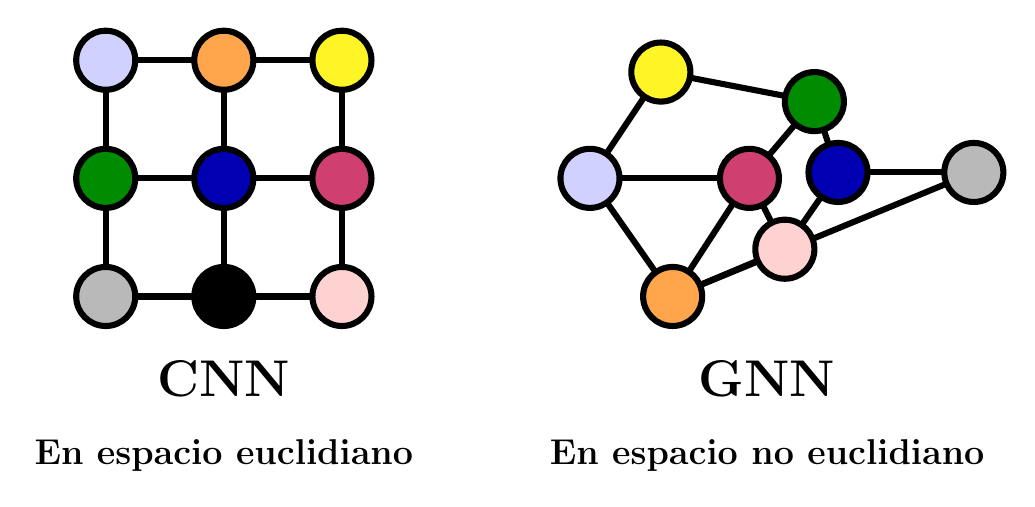
\begin{tikzpicture}[
    scale=0.75,                 % <-- reduce a 3/4
  transform shape,  
  font=\sffamily,
  edge/.style={line width=2.2pt, draw=black},
  v/.style={circle, draw=black, line width=2.2pt, minimum size=10mm, inner sep=0pt},
  title/.style={font=\bfseries\fontsize{28}{28}\selectfont},
  subtitle/.style={font=\bfseries\fontsize{18}{18}\selectfont}
]

% ===================== LEFT: CNN grid =====================
\begin{scope}[shift={(0,0)}]
  % Coordinates (3x3)
  \coordinate (c11) at (0,2);
  \coordinate (c21) at (2,2);
  \coordinate (c31) at (4,2);

  \coordinate (c12) at (0,0);
  \coordinate (c22) at (2,0);
  \coordinate (c32) at (4,0);

  \coordinate (c13) at (0,-2);
  \coordinate (c23) at (2,-2);
  \coordinate (c33) at (4,-2);

  % Edges (grid)
  \draw[edge] (c11)--(c21)--(c31);
  \draw[edge] (c12)--(c22)--(c32);
  \draw[edge] (c13)--(c23)--(c33);

  \draw[edge] (c11)--(c12)--(c13);
  \draw[edge] (c21)--(c22)--(c23);
  \draw[edge] (c31)--(c32)--(c33);

  % Nodes (colores)
  \node[v, fill=blue!18]   at (c11) {};              % azul claro
  \node[v, fill=orange!70] at (c21) {};              % naranja
  \node[v, fill=yellow!85] at (c31) {};              % amarillo

  \node[v, fill=green!55!black] at (c12) {};         % verde oscuro
  \node[v, fill=blue!70!black]  at (c22) {};         % azul oscuro
  \node[v, fill=purple!75]      at (c32) {};         % morado

  \node[v, fill=gray!55]   at (c13) {};              % gris
  \node[v, fill=black]     at (c23) {};              % negro
  \node[v, fill=pink!70]   at (c33) {};              % rosa

  % Labels
  \node[title]    at (2,-3.4) {CNN};
  \node[subtitle] at (2,-4.7) {En espacio euclidiano};
\end{scope}

% ===================== RIGHT: GNN graph =====================
\begin{scope}[shift={(8.2,0)}]
  % Node positions
  \coordinate (r)  at (0,0);       % azul claro (antes rojo)
  \coordinate (y)  at (1.2,1.8);   % amarillo
  \coordinate (g)  at (3.8,1.3);   % verde
  \coordinate (b)  at (4.2,0.1);   % azul oscuro
  \coordinate (gr) at (6.5,0.1);   % gris
  \coordinate (o)  at (1.4,-2.0);  % naranja
  \coordinate (p)  at (2.7,0.0);   % morado
  \coordinate (pk) at (3.3,-1.2);  % rosa

  % Edges
  \draw[edge] (r)--(y);
  \draw[edge] (y)--(g);
  \draw[edge] (g)--(b);
  \draw[edge] (b)--(gr);

  \draw[edge] (r)--(p);
  \draw[edge] (r)--(o);

  \draw[edge] (o)--(p);
  \draw[edge] (p)--(pk);
  \draw[edge] (pk)--(b);

  \draw[edge] (p)--(g);
  \draw[edge] (o)--(pk);

  \draw[edge] (o)--(gr);

  % Nodes (misma paleta que CNN)
  \node[v, fill=blue!18]         at (r)  {};         % azul claro
  \node[v, fill=yellow!85]       at (y)  {};         % amarillo
  \node[v, fill=green!55!black]  at (g)  {};         % verde oscuro
  \node[v, fill=blue!70!black]   at (b)  {};         % azul oscuro
  \node[v, fill=gray!55]         at (gr) {};         % gris
  \node[v, fill=orange!70]       at (o)  {};         % naranja
  \node[v, fill=purple!75]       at (p)  {};         % morado
  \node[v, fill=pink!70]         at (pk) {};         % rosa

  % Labels
  \node[title]    at (3.0,-3.4) {GNN};
  \node[subtitle] at (3.0,-4.7) {En espacio no euclidiano};
\end{scope}

\end{tikzpicture}
\end{figure}




\subsection{Codificación y predicción}
Se utilizan los términos \textit{encoder} y \textit{decoder} para separar la construcción de una representación de su transformación en una predicción. Aquí se considera la tarea de clasificación; no se presupone que el segundo reconstruya la gráfica ni sea una inversa del primero.

\begin{definition}[Encoder]
\label{def:encoder}
Fijadas una gráfica $G=(V,E)$, sus características iniciales y los parámetros del modelo, un \emph{encoder} o codificador de nodos es una aplicación
\[
\phi:V\longrightarrow\mathbb R^d,\qquad \phi(v)=z_v.
\]
El vector $z_v$ es el encaje del nodo $v$. En los codificadores basados en propagación de mensajes, esta representación depende de los atributos de $v$ y de la información que se agrega a través de las adyacencias. La dependencia de la gráfica, los atributos y los parámetros queda implícita al escribir $\phi(v)$.
\end{definition}

\begin{figure}[ht]
\centering
\begin{tikzpicture}[
  font=\sffamily,
  >=Latex,
  nodeG/.style={circle, fill=gray!55, draw=none, minimum size=5.5pt, inner sep=0pt},
  nodeH/.style={circle, fill=gray!15, draw=black, line width=0.6pt, minimum size=10pt, inner sep=0pt},
  edge/.style={line width=0.8pt, draw=black},
  dotarr/.style={densely dotted, line width=1.0pt, -{Latex[length=2.2mm]}},
  labelB/.style={font=\bfseries},
  small/.style={font=\small}
]

% ---------------- LEFT: original network ----------------
% cluster left
\node[nodeG] (a) at (0.0, 0.8) {};
\node[nodeG] (b) at (0.6, 1.2) {};
\node[nodeG] (c) at (0.8, 0.3) {};
\node[nodeG] (d) at (0.2,-0.1) {};
\node[nodeG] (e) at (-0.2,0.3) {};

\draw[edge] (a)--(b)--(c)--(a);
\draw[edge] (a)--(d)--(e)--(a);
\draw[edge] (c)--(d);

% bridge to u,v triangle
\node[nodeG] (m) at (1.5, 0.5) {};
\draw[edge] (c)--(m);

% highlighted triangle (u,v + one more)
\node[nodeH] (u) at (2.2, 0.85) {$u$};
\node[nodeH] (v) at (2.8, 0.55) {$v$};
\node[nodeG] (t) at (2.4, 1.35) {};

\draw[edge] (m)--(u);
\draw[edge] (m)--(v);
\draw[edge] (u)--(v);
\draw[edge] (u)--(t);
\draw[edge] (t)--(v);

% label under left
\node[labelB] at (1.4,-1.0) {Red original};



\coordinate (C) at (7.2,0.85);
\fill[red!35, opacity=0.55] (C) circle (1.75);

% points inside
\node[circle, fill=black, inner sep=1.2pt, label={[small]right:$z_u$}] (zu) at ($(C)+(-0.35,0.75)$) {};
\node[circle, fill=black, inner sep=1.2pt, label={[small]right:$z_v$}] (zv) at ($(C)+(-0.15,0.10)$) {};

% label under right
\node[labelB] at (7.2,-1.0) {Espacio encajado};

% ---------------- Arcs + text ----------------
% dotted arrows from u and v to embedding points
\draw[dotarr] (u) .. controls (4.2,2.0) and (5.6,2.1) .. (zu);
\draw[dotarr] (v) .. controls (4.2,0.3) and (5.7,0.1) .. (zv);

% ENC labels near arcs
\node[small] at (4.1,1.75) {$\phi(u)$};
\node[small] at (4.1,0.25) {$\phi(v)$};

% "encode nodes" label in the middle
\node[small] at (4.55,1.05) {codificar nodos};

\end{tikzpicture}
\end{figure}

Los encajes de los nodos se organizan en una matriz respetando la enumeración usada para $\mathbf X$ y $\mathbf A$. Esto permite expresar varias capas de propagación mediante operaciones matriciales.

\begin{definition}[Matriz de encajes]
\label{def:matriz-encajes}
    Sea $G = (V, E)$ una gráfica, con $|V| = \nu_G$.
    La \emph{matriz de encajes} es una matriz
    \[
        \mathbf{Z} \in \mathbb{R}^{\nu_G \times d}
    \]
    cuyas filas corresponden a los encajes de los vértices.
    Para cada $v \in V$, el vector de encaje asociado se denota por
    \[
        \phi(v) = \mathbf{Z}[v],
    \]
    donde $\mathbf{Z}[v]$ representa la fila de $\mathbf{Z}$ correspondiente al vértice $v$, y $\phi(v) = z_v \in \mathbb{R}^d$ es el vector de encaje del nodo $v$.
\end{definition}
Cada fila contiene información de un nodo. La matriz completa aún no es un único vector que represente la gráfica; para obtenerlo se introducirá una agregación global.

Una vez obtenidos los encajes, una función de predicción los transforma en salidas acordes con la tarea.

\begin{definition}[Decoder]
\label{def:decoder}
Un \emph{decoder} o función de predicción es una aplicación
\[
\psi:\mathbb R^d\longrightarrow\widehat{\mathcal Y}
\]
que transforma un encaje en una predicción. Para una tarea por nodo se escribe $\hat y_v=\psi(z_v)$. Si se utiliza un encaje global de la gráfica, la salida corresponde a la gráfica completa. El espacio $\widehat{\mathcal Y}$ es el espacio de predicciones de la Definición~\ref{def:funcion-perdida}.
\end{definition}

\begin{figure}[H]
\centering
\begin{tikzpicture}[>=Latex,node distance=1.1cm]
\node[draw,rounded corners] (z) {$z_v\in\mathbb R^d$};
\node[draw,rounded corners,right=of z] (dec) {Función de predicción $\psi$};
\node[draw,rounded corners,right=of dec] (out) {$\hat y_v$};
\draw[->] (z)--(dec);
\draw[->] (dec)--(out);
\end{tikzpicture}
\caption{Predicción por nodo a partir de un encaje. Para clasificar la gráfica completa se requiere una representación global previa.}
\end{figure}

Estas funciones separan representación y predicción. La siguiente construcción especifica cómo obtener los encajes mediante información de los vecindarios.

\subsection{Propagación de Mensajes Neuronales}
La propagación de mensajes actualiza el estado de cada nodo a partir de su estado anterior y de los estados de sus vecinos. Se fija $h_v^{(0)}=x_v$, donde $x_v$ es el vector de atributos iniciales de $v$. Los estados de una capa se calculan utilizando los de la capa anterior; no se mezclan actualizaciones de la misma iteración.

\begin{definition}[Propagación de mensajes neuronales]
\label{def:propagacion-mensajes}
Sea $G=(V,E)$ y, para $t\geq1$, sean $h_u^{(t-1)}$ los estados de los nodos en la capa anterior. Una forma básica de mensaje agregado en el nodo $v$ es
\[
m_v^{(t)}=\mathscr A\bigl((h_u^{(t-1)})_{u\in N_G(v)}\bigr),
\]
donde $\mathscr A$ combina una familia de vectores sin depender de su orden. La familia conserva multiplicidades: dos vecinos con el mismo estado siguen aportando dos elementos. Ejemplos son la suma, el promedio y el máximo componente a componente. Para un vecindario vacío debe fijarse una convención; en la suma se utiliza el vector cero.
\end{definition}

El mensaje agregado se combina con el estado previo del nodo central mediante una función de actualización.

\begin{definition}[Actualización de estados neuronales]
\label{def:actualizacion-estados}
    Sea $h_v^{(t-1)}$ el encaje oculto del nodo $v$ en la capa anterior $(t-1)$, y $m_v^{(t)}$ el mensaje agregado en la capa $t$. Entonces, la actualización del estado del nodo está dada por:
    \[
        h_v^{(t)} = \mathscr{U}\!\left(h_v^{(t-1)},\, m_v^{(t)}\right),
    \]
    donde $\mathscr{U}$ es una función de actualización, típicamente implementada mediante una red neuronal, por ejemplo, una capa lineal seguida de una función de activación (como ReLU).
\end{definition}

Tras $K$ iteraciones, el estado final define el encaje del nodo:

\begin{center}
    $z_u$ = $h_u^{(K)}$.
\end{center}

La Figura~\ref{fig:gnn-message-passing-formal} reúne ambas operaciones. Si cada capa utiliza únicamente vecinos inmediatos, tras $K$ capas el estado de un nodo puede depender de atributos situados a lo más a $K$ aristas de distancia. Esto expresa un alcance combinatorio, no una garantía de recuperar invariantes topológicos de la superficie.

\begin{figure}[H]
\centering
\resizebox{\textwidth}{!}{
\begin{tikzpicture}[ 
    font=\small\sffamily, 
    >=Latex, 
    every node/.style={align=center}, 
    main/.style={ 
        circle, 
        draw=black, 
        very thick, 
        minimum size=1cm, 
        inner sep=2pt, 
        fill=blue!15 
        }, 
    neigh/.style={ 
        circle, 
        draw=black, 
        thick, 
        minimum size=0.9cm, 
        inner sep=2pt, 
        fill=gray!15 
        }, 
    box/.style={ 
        rounded corners=3pt, 
        draw=black, 
        thick, 
        fill=white, 
        minimum height=0.9cm, 
        minimum width=3cm, 
        inner sep=4pt 
        }, 
    smallbox/.style={ 
        rounded corners=3pt, 
        draw=black, 
        thick, 
        fill=white, 
        minimum height=0.7cm, 
        minimum width=2.7cm, 
        inner sep=3pt 
        }, 
    lab/.style={ 
        font=\footnotesize 
        }, 
    flow/.style={ 
        ->, very thick, 
        shorten >=2pt, 
        shorten <=2pt 
        } 
    ] 
    \node[main] (v) at (0,0) 
    {$v$\\[-1mm]\scriptsize $h_v^{(t-1)}$}; 
    \node[neigh] (u1) at (-1.8,1.4) 
    {$u_1$\\[-1mm]\scriptsize $h_{u_1}^{(t-1)}$}; 
    \node[neigh] (u2) at (-1.9,-1.4) 
    {$u_2$\\[-1mm]\scriptsize $h_{u_2}^{(t-1)}$}; 
    \node[neigh] (u3) at (1.8,1.4) 
    {$u_3$\\[-1mm]\scriptsize $h_{u_3}^{(t-1)}$}; 

    % ----------------------------- 
    % Graph edges and message flow 
    % ----------------------------- 

    \draw[ 
        ->, 
        very thick, 
        blue!70, 
        shorten >=3pt, 
        shorten <=3pt 
        ] 
    (u1) -- (v); 
        
    \draw[ 
        ->, 
        very thick, 
        blue!70, 
        shorten >=3pt, 
        shorten <=3pt 
        ] 
    (u2) -- (v); 
    
    \draw[ 
        ->, 
        very thick, 
        blue!70, 
        shorten >=3pt, 
        shorten <=3pt 
        ] 
    (u3) -- (v); 

    % Neighborhood label 
    \node[lab] at (0,-2.2) 
    {$N_G(v)=\{u_1,u_2,u_3\}$};

     % ----------------------------- 
     % Aggregation block 
     % ----------------------------- 
     \node[box] (agg) at (5,0) { 
        $\displaystyle m_v^{(t)} = \mathscr{A} \bigl( (h_u^{(t-1)})_{u\in N_G(v)} \bigr) $
        }; 
    \draw[flow] (v.east) -- (agg.west); 
    
    % ----------------------------- 
    % Update block 
    % ----------------------------- 
    
    \node[box] (upd) at (9.5,0) { 
        $\displaystyle h_v^{(t)} = \mathscr{U} \left( h_v^{(t-1)}, m_v^{(t)} \right) $ 
        }; 
    \draw[flow] (agg.east) -- (upd.west); 
    % ----------------------------- 
    % Updated node 
    % ----------------------------- 
    
    \node[ main, fill=green!18 ] (newv) at (12.8,0) {
        $v$\\[-1mm]\scriptsize $h_v^{(t)}$
        }; 
    \draw[flow] (upd.east) -- (newv.west); 

    % ----------------------------- 
    % Final embedding 
    % ----------------------------- 
    
    \node[smallbox] (final) at (9.5,-1.8) { 
        $\displaystyle z_v=h_v^{(K)}$ 
        }; 

    \node[lab] at (9.5,-2.65) {Representación final del nodo tras $K$ iteraciones}; 
    
    \draw[ 
        ->, 
        thick, 
        dashed, 
        rounded corners, 
        shorten >=2pt, 
        shorten <=2pt 
        ] 
        
    (newv.south) |- (final.east); 

        % ----------------------------- 
        % Step annotations 
        % ----------------------------- 
        \node[lab, anchor=west] at (-2.7,2.4) {
            \textbf{Iteración \(t\):} Propagación local
            }; 
            
        \node[lab] at (5,1.8) {
            \textbf{1.} Agregación
            
            }; 
            
            \node[lab] at (9.5,1.8) {
                \textbf{2.} Actualización
                }; 
            
            \end{tikzpicture} }
\caption{Esquema del mecanismo de propagación de información en una red neuronal sobre gráficas. En la iteración \(t\), cada nodo \(v\) agrega las representaciones de sus vecinos mediante una función invariante al orden \(\mathscr{A}\), obteniendo \(m_v^{(t)}\). Posteriormente, su representación se actualiza mediante \(\mathscr{U}\), combinando el estado previo con la información agregada. Tras \(K\) iteraciones, se obtiene la representación final \(z_u = h_u^{(K)}\), que captura información de los atributos y las adyacencias.}
\label{fig:gnn-message-passing-formal}
\end{figure}
\newpage
\subsection{La GNN fundamental}

La agregación anterior puede ampliarse transformando primero cada par de estados del nodo central y de un vecino. Esta formulación distingue la función que produce mensajes de la que actualiza el estado, y sirve como antecedente de las operaciones locales presentadas en el Capítulo~\ref{cap:resultados}.

\begin{definition}[Modelo GNN fundamental]
\label{def:gnn-fundamental}
Sean $x_u\in\mathbb R^{d_0}$ los atributos del nodo $u$, $\mathscr M:\mathbb R^{d_0}\times\mathbb R^{d_0}\to\mathbb R^r$ una función de mensajes y $\mathscr U:\mathbb R^{d_0}\times\mathbb R^r\to\mathbb R^{d_1}$ una función de actualización. Una capa de propagación puede escribirse como
\[
h_u=\mathscr U\!\left(x_u,\,\bigoplus_{v\in N_G(u)}\mathscr M(x_u,x_v)\right),
\]
donde $\bigoplus$ agrega, sin depender del orden, la familia de mensajes indexada por los vecinos. Esta familia conserva las multiplicidades. Las funciones $\mathscr M$ y $\mathscr U$ comparten sus parámetros entre los nodos de la capa.
\end{definition}

La operación comprende tres pasos: producir un mensaje por vecino, agregar esos mensajes y actualizar el nodo central. La notación $\mathscr M$ y $\mathscr U$ distingue estos componentes del codificador $\phi$ y del predictor $\psi$. En capas posteriores se sustituyen los atributos iniciales por los estados de la capa anterior. Cuando se usan promedio o máximo, debe especificarse el tratamiento de nodos aislados o incluirse al propio nodo en la agregación.

\subsection{Arquitectura y simetrías de una GNN}

La forma matricial organiza simultáneamente las actualizaciones de todos los nodos y permite precisar el papel de la entrada que se modifica en el Capítulo~\ref{cap:muestreo}.

\begin{definition}[Arquitectura de una GNN]
\label{def:arquitectura-gnn}
Sean $\mathbf A\in\mathbb R^{\nu_G\times\nu_G}$ la matriz de adyacencia y $\mathbf H_0=\mathbf X\in\mathbb R^{\nu_G\times d_0}$ la matriz de características iniciales. Una GNN con $K$ capas de propagación se expresa como
\[
\mathbf H_{t+1}=\mathbf F(\mathbf H_t,\mathbf A,\Phi_t),
\qquad t=0,\ldots,K-1,
\]
donde $\mathbf H_t\in\mathbb R^{\nu_G\times d_t}$, $\Phi_t$ contiene los parámetros de la capa y $\mathbf F$ combina mensajes y actualización con dimensiones compatibles. La notación $\mathbf F$ representa la operación de cada capa, cuyos parámetros y dimensiones pueden variar con $t$. La matriz final $\mathbf H_K$ es la matriz de encajes de la Definición~\ref{def:matriz-encajes}.
\end{definition}

Esta formulación utiliza una adyacencia fija. En modelos que reconstruyen sus conexiones durante las capas se requiere una matriz $\mathbf A_t$ dependiente del estado; tal es la distinción que se retomará al presentar DGCNN. Cambiar la matriz de entrada mediante muestreo tampoco equivale a aprender nuevas características: son operaciones diferentes.

La equivarianza de la Definición~\ref{def:equivarianza} se especializa ahora a la enumeración de nodos. Al cambiar esa enumeración, deben permutarse de forma compatible tanto las características como la adyacencia.

\begin{definition}[Equivarianza a permutaciones]
\label{def:equivarianza-permutaciones}
Sean $\mathbf H\in\mathbb R^{\nu_G\times d}$, $\mathbf A\in\mathbb R^{\nu_G\times\nu_G}$ y $\mathbf P\in\mathbb R^{\nu_G\times\nu_G}$ una matriz de permutación. Una capa $\mathbf F$ es \textbf{equivariante a permutaciones} si, para toda entrada admisible y toda $\mathbf P$,
\[
\mathbf F(\mathbf P\mathbf H,\mathbf P\mathbf A\mathbf P^T,\Phi)
=\mathbf P\,\mathbf F(\mathbf H,\mathbf A,\Phi).
\]
La multiplicación por $\mathbf P$ a la izquierda reordena las filas, que corresponden a los nodos. La salida se reordena de la misma manera; no permanece necesariamente igual como matriz.
\end{definition}

La propagación con funciones compartidas y agregación independiente del orden respeta este cambio de enumeración: cada nodo recibe la misma familia de mensajes, sólo reindexada. Esta propiedad de las capas no se transfiere automáticamente al procedimiento de reducción del Capítulo~\ref{cap:muestreo}, cuyas decisiones también dependen del recorrido y de los índices.

Para clasificar una gráfica completa se utiliza una agregación global $\mathscr R$ sobre los encajes, seguida de una función predictora:
\[
z_G=\mathscr R\bigl((z_v)_{v\in V}\bigr),\qquad
\hat y_G=\psi(z_G).
\]
Si $\mathscr R$ es independiente del orden, por ejemplo una suma o un máximo componente a componente, y los encajes son equivariantes, la predicción es invariante a la enumeración. Así se distingue la representación por nodo de la representación global necesaria para clasificar una superficie.

\section{Redes gráficas convolucionales (GCN)}

Una GCN es un caso particular de GNN que utiliza una agregación convolucional sobre la gráfica. Para concretar esta diferencia, se considera la agregación normalizada por grados descrita en \cite{graph_representation_learning}. Sean
\[
\widetilde{\mathbf A}=\mathbf A+\mathbf I,\qquad
\widetilde{\mathbf D}_{ii}=\sum_j\widetilde{\mathbf A}_{ij},
\]
donde $\mathbf I$ es la identidad y $\widetilde{\mathbf D}$ es diagonal. La identidad incorpora el estado propio del nodo en la propagación; $\widetilde{\mathbf A}$ no es la matriz de adyacencia de la gráfica simple original. Esta construcción usa el grado de la Definición~\ref{def:grado-vertice} y permite definir una capa mediante
\[
\mathbf H_{t+1}=\sigma\!\left(
\widetilde{\mathbf D}^{-1/2}\widetilde{\mathbf A}
\widetilde{\mathbf D}^{-1/2}\mathbf H_t\mathbf W_t
\right).
\]
Aquí $\mathbf W_t\in\mathbb R^{d_t\times d_{t+1}}$ transforma las características, la matriz normalizada combina vecinos y $\sigma$ actúa componente a componente. Los pesos multiplican a la derecha porque cada nodo ocupa una fila, a diferencia de la convención de vectores columna usada en las capas densas. La Figura~\ref{fig:graph_convolutions} ilustra el intercambio local de información.

\begin{figure}[ht]
\centering
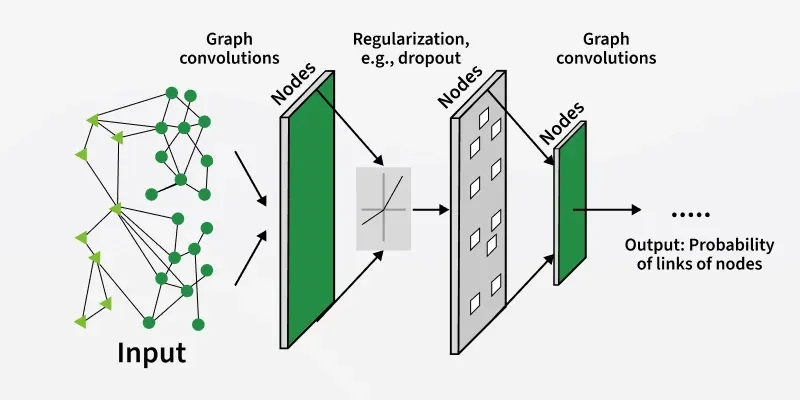
\includegraphics[width=0.6\textwidth]{img/graph_convolutions.jpg}
\caption{Ilustración de la agregación local de información sobre una gráfica.}
\label{fig:graph_convolutions}
\end{figure}

Los fundamentos anteriores permiten distinguir las entradas y las operaciones de los modelos estudiados en el Capítulo~\ref{cap:resultados}. PointNet procesa conjuntos de puntos mediante transformaciones compartidas y agregación simétrica \cite{pointnet}; no requiere propagación sobre una matriz de adyacencia. Las GNN emplean relaciones entre nodos y las GCN constituyen una familia particular dentro de ellas. Por su parte, FNO se presenta como un operador neuronal, no como una GCN. Las arquitecturas específicas se desarrollarán allí, sin identificar automáticamente todos los modelos sobre datos geométricos con redes gráficas.

El Capítulo~\ref{cap:muestreo} utiliza estas distinciones para transformar las coordenadas y adyacencias de entrada antes del aprendizaje. La evaluación posterior examina el efecto de esa representación en la clasificación; ni la equivarianza de una capa ni una predicción acertada demuestran, por sí solas, que la reducción conserve la topología de la superficie.
